%

%\NeedsTeXFormat{LaTeX2e}[1996/06/01]
 
\documentclass[12pt]{article}
\usepackage{epsf}
\usepackage{amssymb}
\usepackage{graphicx}  
\usepackage{ucs}
\usepackage[utf8x]{inputenc}
\usepackage[libertine]{newtxmath}

\usepackage{bm}

\usepackage{geometry}
 \geometry{
 a4paper,
 total={167mm,244mm},
 left=24mm,
 top=22mm,
 }

\usepackage{amsmath}
\usepackage{empheq}

\newlength\dlf  % Define a new measure, dlf
\newcommand\alignedbox[2]{
% Argument #1 = before & if there were no box (lhs)
% Argument #2 = after & if there were no box (rhs)
&  % Alignment sign of the line
{
\settowidth\dlf{$\displaystyle #1$}  
    % The width of \dlf is the width of the lhs, with a displaystyle font
\addtolength\dlf{\fboxsep+\fboxrule}  
    % Add to it the distance to the box, and the width of the line of the box
\hspace{-\dlf}  
    % Move everything dlf units to the left, so that & #1 #2 is aligned under #1 & #2
\boxed{#1 #2}
    % Put a box around lhs and rhs
}
}
 
\bibliographystyle{plain}
\usepackage{bm}
\usepackage{amsfonts}
\usepackage{amsmath}
\usepackage{mathrsfs}
\RequirePackage{epsf}
\RequirePackage{longtable}
%\usepackage{times}



\def\d{\delta}
\def\n{\nabla}
\def\l{\lambda}
%\def\e{\epsilon}
\def\ep{\epsilon}
\def\D{\Delta}
\def\p{\partial}
\def\s{\mathfrak s}
%\def\pmb#1{\setbox0=\hbox{#1}%
\def\til#1{#1 \atop \tilde{\phantom{a}}}

%SF-98%
\def\ri{\right}
\def\le{\left}
\def\o{\omega}
\def\f{\phi}
\def\p{\psi}
\def\a{\alpha}
\def\b{\beta}
\def\g{\gamma}
\def\t{\theta}
\def\r{\frac{1}{r}}
\def\sr{\frac{1}{r^2}}
\def\nn{\nonumber}
\def\oh{\frac{1}{2}}
\def\Lie{{\cal L}}
\def\be{\begin{equation}}
\def\ee{\end{equation}}
\def\ba{\begin{eqnarray}}
\def\ea{\end{eqnarray}}
\def\twothirds{\hbox{$\,^2\!/_3$}}
\def\<{\noindent }
%\def\dis{$\displaystyle}
%%%%%%%

%SUF-PD-04%
\newcommand{\beq}{\begin{equation}}
\newcommand{\eeq}{\end{equation}}
\newcommand{\beqn}{\begin{eqnarray}}
\newcommand{\eeqn}{\end{eqnarray}}
\newcommand{\beaa}{\begin{eqnarray*}}
\newcommand{\eeaa}{\end{eqnarray*}}
%\newcommand{$\displaystyle}{$\displaystyle}
%\newcommand{\Lie}{\mbox{\pounds}}
\newcommand{\pa}{\partial}
\newcommand{\na}{\nabla}
\newcommand{\vp}{\varphi}
\def\Madm{M_{\rm ADM}}
\def\Jadm{J_{\rm ADM}}
\def\Mchi{M_{\rm \chi}}
\def\Mmix{M_{\rm mix}}
\def\MK{M_{\rm K}}
\newcommand{\rhoH}{\rho_H}
\newcommand{\HG}{{\cal H}_G}
\newcommand{\CG}{{\cal C}_G}

\def\2pi{2\pi}
\def\zero{\hbox{$_{(0)}$}}
\def\bL{\hbox{$\,{\cal L}\!\!\!\!\!-$}}
\def\bI{\hbox{$\,I\!\!\!\!-$}}
%%%\def\zeroD{\hbox{$\,D\!\!\!\!\!\!^{(0)}$}}
%%%%\def\zeroD{\stackrel{{\scriptsize{(0)}}}{D}}
%%%%\def\fourR{\stackrel{{\scriptsize{(4)}}}{R}}
%%%%\def\zeroDelta{\stackrel{{\scriptsize (0)}}{\Delta}}
\def\zeroD{\stackrel{{(0)}}{D}}
\def\fourR{\stackrel{{(4)}}{R}}
\def\zeroDelta{\stackrel{(0)}{\Delta}}
\def\two{\hbox{$^{(2)}$}}
\def\three{\hbox{$^{(3)}$}}
\def\four{\hbox{$^{(4)}$}}
\def\tn{\hbox{$^{(n)}$}}
%%%
\newcommand{\gab}{g_{\alpha\beta}}
\newcommand{\gabu}{g^{\alpha\beta}}
\newcommand{\gabd}{g_{\alpha\beta}}
\newcommand{\gmabu}{\gamma^{ab}}
\newcommand{\gmabd}{\gamma_{ab}}
\newcommand{\tgmabu}{\tilde\gamma^{ab}}
\newcommand{\tgmabd}{\tilde\gamma_{ab}}
%\newcommand{\th}{\tilde h}
\newcommand{\tgamma}{\tilde\gamma}
\newcommand{\thh}{\tilde h}
\newcommand{\tf}{\tilde f}
\newcommand{\piabu}{\pi^{ab}}
\newcommand{\piabd}{\pi_{ab}}
\newcommand{\piab}{\pi_a{}^b}
\newcommand{\tpiabu}{\tilde{\pi}^{ab}}
\newcommand{\tpiabd}{\tilde{\pi}_{ab}}
\newcommand{\tpi}{\tilde{\pi}}
\newcommand{\qab}{q_\alpha{}\!^\beta}
\newcommand{\qbc}{q_\beta{}\!^\gamma}
\newcommand{\qabu}{q^{\alpha\beta}}
\newcommand{\qabd}{q_{\alpha\beta}}
\newcommand{\Tabd}{T_{\alpha\beta}}
\newcommand{\Tabu}{T^{\alpha\beta}}
\newcommand{\Tab}{T^\alpha{}\!_\beta}
\newcommand{\Gab}{G^\alpha{}\!_\beta}
\newcommand{\Gabd}{G_{\alpha\beta}}
\newcommand{\Gabu}{G^{\alpha\beta}}
\newcommand{\Rab}{R^\alpha{}\!_\beta}
\newcommand{\dSab}{dS_{\alpha\beta}}
\newcommand{\dSa}{dS_{\alpha}}
\newcommand{\QK}{Q_{\rm K}}
\newcommand{\dl}{\delta}
\newcommand{\dlab}{\dl^\alpha{}\!_\beta}
\newcommand{\dlabu}{\dl_\alpha{}\!^\beta}
\newcommand{\dlgab}{\delta g_{\alpha\beta}}
\newcommand{\Dlgab}{\Delta g_{\alpha\beta}}
\newcommand{\Dlgabu}{\Delta g^{\alpha\beta}}
\newcommand{\Dl}{\Delta}
\newcommand{\dw}{\ \,}
\newcommand{\dww}{\ \,\,}
\newcommand{\Lag}{{\mathscr L}}
%% Macros for action and trivials
\def\a{\alpha}
\def\b{\beta}
\def\c{\gamma}
\def\d{\delta}
\def\e{\zeta}
\def\f{\eta}
\newcommand{\bsube}{\begin{subequations}}
\newcommand{\esube}{\end{subequations}}
%
\newcommand{\gmaa}{\gamma_a\!{}^\alpha}
\newcommand{\zD}{{\raise1.0ex\hbox{${}^{\ \circ}$}}\!\!\!\!\!D}
\newcommand{\zLap}{{\raise1.0ex\hbox{${}^{\ \circ}$}}\!\!\!\!\Delta}
\newcommand{\upp}[2]{{\raise0.9ex\hbox{${}^{\ #2}$}}\!\!\!\!#1\,}
\newcommand{\up}[2]{{\raise0.4ex\hbox{${}^{\ #2}$}}\!\!\!#1\,}
%\newcommand{\bigdotxi}{{\raise0.8ex\hbox{${}^{\ \mbox{\tiny$\bullet$}}$}}\!\!\!\xi}
\newcommand{\bigdotxi}{\bm\dot{\mit\xi}}
\newcommand{\ap}{\frak a}
\newcommand{\bp}{\frak b}
\newcommand{\ylm}{Y_{l m}}
\newcommand{\apj}{Astrophysical J.}
\newcommand{\mnras}{MNRAS}
%%% Appendix macros
%\newcommand{\bea}{\begin{eqnarray}} 
%\newcommand{\eea}{\end{eqnarray}}
\def\bea{\begin{eqnarray}}
\def\eea{\end{eqnarray}}
\newcommand{\dis}{\displaystyle}
%\newcommand{\ep}{\epsilon}
\newcommand{\cancel}[2]{\underline{#1}\begin{picture}(0,0)\put(#2,-1){{}$_{{}_/}$}\end{picture}}
\newcommand{\cancell}[2]{\underline{#1}\begin{picture}(0,0)\put(#2,-1){{}$_{{}_/\!_/}$}\end{picture}}
%%%
\def\dflat{\hbox{$\nabla$\kern-.6em\hbox{\raise.27em\hbox{\tiny$\backslash$}}} }
\newcommand{\boldnabla}{\mbox{\boldmath$\nabla$}}
\makeindex
\usepackage[normalem]{ulem}

\begin{document}


\begin{center}
{\large \bf Lecture Notes on Relativistic Stars} \\
\hspace{1cm}\\
 {\large Nikolaos Stergioulas} \\
 \vskip0.2cm
  Department of Physics\\ Aristotle University of Thessaloniki
\end{center}

\section*{Preface}

These lecture notes are distributed as part of the teaching material for the GR course in the MSc program at the Aristotle University of Thessaloniki.

\section*{Conventions}
\index{conventions}

Gravitational units ($G = c = 1)$ are used in equations,  while numerical results are listed in appropriate units (cgs, km, $M_\odot$ etc.).  The signature of the spacetime
metric is $(-+++)$. Abstract spacetime indices are Greek, $\alpha$, $\beta,
\ldots$, while spatial indices are Latin $a, b, \ldots$.
Indices $\mu, \nu, \lambda$ and
$i,j,k$ will be concrete, taking values $\mu = 0,1,2,3$, $i=1,2,3$ etc.


Numbers that rely on physical constants are based on the values
%\hfil\break
$c = 2.9979  \times10^{10}\ $cm$\ $s$^{-1}$, \enskip
$G = 6.670\times10^{-8} $g$^{-1} $cm$^{3} $s$^{-2}$, \enskip
$\hbar = 1.0545\times10^{-27} $g cm$^{2}$s$^{-1}$, \enskip
baryon mass $m_B = 1.659\times 10^{-24}$g, and
$M_\odot = 1.989\times10^{33}$g $ = 1.477$ km.


%%%%%%%%%%%%%%%%%%%%%%%%%%%%%%%%%%%%%%%%%%%%%%%%%%%%%%%%%%%%%%%%%%%%%%%%%%%
%%%%%%%%%%%%%%%%%%%%%%%%%%%%%%%%%%%%%%%%%%%%%%%%%%%%%%%%%%%%%%%%%%%%%%%%%%%

%%%%%%%%%%%%%%%%%%%%%%%%%%%%%%%%%%%%%%%%%%%%%%%%%%%%%%%%%%%%%%%%%%%%%%%%%%%
%%%%%%%%%%%%%%%%%%%%%%%%%%%%%%%%%%%%%%%%%%%%%%%%%%%%%%%%%%%%%%%%%%%%%%%%%%%
\label{chap1}

 \vskip0.4cm

%%%%%%%%%%%%%%%%%%%%%%%%%
\section{Perfect fluids}
%%%%%%%%%%%%%%%%%%%%%%%%%
\label{s:pf}
\noindent
{\it \uline{The stress-energy tensor}.}
  In a perfect fluid one assumes  that a mean velocity field $u^\alpha$ and a mean
stress-energy tensor $T^{\alpha\beta}$ can be defined in fluid elements small compared to the macroscopic length scale but
large compared to the mean free path.  An
observer moving with the average velocity $u^\alpha$ of the fluid will
see the collisions randomly distribute the nearby particle velocities
so that the particle distribution will appear locally isotropic.
Therefore, the components of the fluid's energy
momentum tensor in frame of a comoving observer must have no preferred direction and
$T^{\alpha\beta}u_\beta$ must be invariant under rotations that fix
$u^\alpha$.
It follows that the only nonzero parts of $T^{\alpha\beta}$ are
the rotational scalars
\be
        \epsilon := T^{\alpha\beta} u_\alpha u_\beta,
\end{equation}
and
\be
        p := \frac13 q_{\gamma\delta}T^{\gamma\delta},
\end{equation}
where $q_{\gamma\delta}= g_{\gamma\delta}+u_\gamma u_\delta$ is the projection tensor normal to the fluid.
For such an isotropic, ideal fluid the  stress-energy tensor 
takes the form
\be
\boxed{T^{\alpha\beta} = \epsilon u^\alpha u^\beta + pq^{\alpha\beta}}.
\index{perfect fluid!stress-energy tensor}\index{stress-energy tensor!perfect fluid}
\index{energy-momentum tensor}
\label{Tab}
\ee
%
The scalars $\epsilon$ and $p$ are the {\it energy density}\index{energy density|textbf}
 and the {\it pressure}\index{pressure|textbf}, as measured by a
\textit{comoving} observer.

\vskip0.8cm

\noindent
{\it \uline{Thermodynamics}.}
We denote by $n$ the baryon number density.
The rest-mass density (baryon-mass density)\index{rest-mass density|textbf}\index{baryon!baryon-mass density|textbf} is then
\be
\rho := m_B n, \label{rhoi}
\ee
where $m_B$ is the mass per baryon. We restrict
attention to the case of a perfect fluid with equilibrium 
composition, where the $\epsilon$ and $p$ depend
on  $\rho$ and the {\it specific entropy} 
(entropy per unit rest mass) $s$,
\be
\epsilon = \epsilon(\rho,s),\hskip6em\relax p = p(\rho,s)
\label{eqsti},
\ee
(or, on equivalent sets of parameters). The thermodynamics\index{thermodynamics} of the fluid is described by the first law\index{thermodynamics!first law}, which takes the form
\be
\boxed{d\epsilon = \rho Tds + h d\rho},
\label{ilaw}
\ee
where $T$ is {\it temperature} and $h$ is the 
{\it specific enthalpy} (enthalpy per unit rest mass), 
\be
\boxed{h := {{\epsilon + p}\over \rho}}. \label{enthi}
\index{enthalpy!relativistic|textbf}\ee

\vskip 0.5cm
\textbf{Exercise 1.1:} Derive (\ref{ilaw}) from its more common form
in terms of extensive quantities
\be
dE = TdS - p\,dV+\mu\, dN \equiv TdS - p\,dV + g\, dM_0,
\label{Ilaw}\ee
by introducing the energy $E$, entropy $S$, 
volume $V$, baryon number $N$, and rest mass $M_0=m_BN$
of a fluid element as measured by a comoving observer. Here 
$\mu=gm_B$, where 
 $g =\frac{\epsilon+p}\rho -Ts$ is the \textit{Gibbs free energy}.  

\vskip 0.5cm

The {\it specific internal energy}
(internal energy per unit rest mass) $e$ is defined by the relation
\be
e = \frac{\epsilon}{\rho}-1.
\label{eq:specific-e}\ee
The {\it Newtonian expression for the specific enthalpy} is\be
h_{\rm Newtonian} = h -1= e + p/\rho. \label{eq:enthnewt1}
\ee
and differs from the relativistic enthalpy $h$ because the relativistic energy density $\epsilon$ includes the 
rest-mass density $\rho$.

\vskip0.8cm

\noindent
{\it \textit{\uline{Baroclinic flow}}.}\index{baroclinic|textbf}
From the definition (\ref{enthi}) and using (\ref{ilaw}), one finds
\begin{subequations}
\begin{align}
   dh &= \frac{d\epsilon}\rho+\frac{dp}\rho - \frac{\epsilon+p}{\rho^2}d\rho
        =T ds+ h\frac{d\rho}\rho + \frac{dp}\rho - h\frac{d\rho}\rho, \nonumber\\
         &= T ds +\frac{dp}{\rho}, \nonumber\\
\Rightarrow \ \ \ \ \ \ \ \ \ \ \   \alignedbox{d \ln h}{= \frac{T}{h} ds +\frac{dp}{\epsilon+p}},
\label{dhdpS}
\end{align}
\end{subequations}
implying
\be
\nabla_\a \ln h = \frac{T}{h} \nabla_\a s +\frac{1}{\epsilon+p} \nabla_\a p.
\label{pilnh}
\ee

\vskip 0.5cm
\textbf{Exercise 1.2:} Taking the curl of (\ref{pilnh}), show that 
 in the presence of entropy gradients
($\nabla s \neq 0$), surfaces of constant energy density ({\it isopycnic 
surfaces})\index{isopycnic|textbf} do not, in general, coincide with surfaces of constant pressure ({\it isobaric
surfaces})\index{isobaric|textbf}. Such a flow is called {\it baroclinic} and, for a rotating star, it implies the presence of {\it meridional circulation}.

\vskip0.8cm

\noindent
{\it \uline{Barotropic flow}.}\index{barotropic|textbf}
Within a short time after
formation, neutrino emission cools a newly born neutron star to $10^{10} K \simeq 1$
MeV, which is much smaller than the Fermi energy
of the interior,  $E_{F}
(0.16\,
{\rm fm}^{-3}) \approx 60\, \rm MeV$.  A neutron star is in this sense
cold, and, because nuclear reaction times are shorter than the cooling
time, one can use a zero-temperature {\it equation of state} (EOS) to
describe the matter:
\be
\epsilon = \epsilon (\rho), \quad p =p(\rho),\label{oneparam}
\ee
or, equivalently,
\be
\epsilon = \epsilon (p).
\label{eq:eos1}\ee

A one-parameter equation 
of state of the form (\ref{eq:eos1}) holds, also in more
general situations, such as when the specific entropy is constant throughout
the star ($\nabla s = 0$,  {\it homentropic flow)}\index{homentropic|textbf}. 
or even when $s=s(\rho$), so that effectively the energy density still depends on one parameter only. In such cases, the isopycnic and
isobaric surfaces coincide and the flow is {\it barotropic}.


In a homentropic star, the first law, (\ref{ilaw}), takes the form
\be
   d\epsilon = h d\rho, 
\label{dedrho}\ee
and using (\ref{dhdpS}) the specific enthalpy\index{enthalpy!relativistic} is also given by
\be
    h = \exp\left(\int_0^p \frac{dp}{\epsilon+p}\right),
\label{enth2}\ee 
(notice that  $\dis \epsilon/\rho = 1$ at $p = 0$, since the gas is nonrelativistic at low densities).  


\vskip0.8cm

\noindent
{\it \uline{Conservation of baryons}.}\index{conservation laws!baryons}\index{baryon!baryon conservation}
The baryon mass $ M_0$ of a fluid element is conserved by the motion
of the fluid. The proper volume of a fluid element is the volume $ V$
of a slice orthogonal to $u^\alpha$ through the history of the fluid
element; and conservation of baryons can be written in the form
$ 0 = \Delta M_0 = \Delta (\rho V)$.
The fractional change in $ V$ in a proper time $ \Delta \tau$ is
given by the 3-dimensional divergence of the velocity, in the subspace
orthogonal to $ u^\alpha$:
\be
  \frac{\Delta V}V = q^{\alpha\beta}\nabla_\alpha u_\beta \Delta \tau.
\label{eq:divu1}\ee
Because $ u^\beta u_\beta = -1$, we have
$ u^\beta \nabla_\alpha u_\beta = \frac12 \nabla_\alpha( u_\beta
u^\beta)
 = 0$, implying
\be
q^{\alpha\beta}\nabla_\alpha u_\beta = \nabla_\beta u^\beta.
\label{eq:divu2}\ee
With $\displaystyle u^\alpha \nabla_\alpha \rho = \frac d{d\tau}\rho$,
conservation of baryons takes the form
\be 0 = \frac{\Delta(\rho V)}V
= \Delta\rho+\rho\frac{\Delta V}V
= (u^\alpha\nabla_\alpha\rho + \rho \nabla_\alpha u^\alpha)\Delta
\tau,
\label{drhodv}\ee
or
\be
       \boxed{ \nabla_\alpha (\rho u^\alpha) = 0}.
\label{eq:baryon}\ee

\vskip 0.8cm
\noindent{\it \uline{Conservation of stress-energy tensor}.} The Bianchi identities and the Einstein field equations  imply that the
stress-energy
tensor is conserved
\be \nabla_\beta T^{\alpha\beta} = 0. \label{divT}\ee
By projecting this conservation along the fluid velocity and normal to it, one obtains separate equations for the conservation of energy and momentum. 

\vskip0.5cm

\textbf{Exercise 1.3:} Show that the projection along the fluid velocity  $ u_\alpha\nabla_\beta T^{\alpha\beta} = 0$
leads to 
\begin{equation}
\boxed {\nabla_\beta (\epsilon u^\beta ) = -p\nabla_\beta u^\beta}.
\label{econs}
\end{equation}
(\textit{conservation of energy}) and that the projection normal to the fluid velocity
$q^\alpha{}_\gamma \nabla_\beta T^{\beta\gamma} = 0$
 leads to 
\begin{equation}
\boxed{ (\epsilon +p)u^\beta\nabla_\beta u^\alpha
        = -q^{\alpha\beta}\nabla_\beta p},
\label{eq:euler}
\end{equation}
(\textit{conservation of momentum} or equations of motion).

\vskip0.5cm

\textbf{Exercise 1.4:} For a barotropic fluid with constant entropy (a homentropic fluid) write the relativistic Euler equation in the form 
\be
   u^\beta\nabla_\beta u^\alpha = -q^{\alpha\beta}\nabla_\beta\ln h.
\label{eq:euler1}\ee
or, equivalently,
\be
    u^\b \omega_{\alpha\beta} = 0,
\label{eq:euler1a}\ee
where\be
\omega_{\alpha\beta} = \nabla_\alpha ( h\,u_\beta )  -
  \nabla_\beta ( h\,u_\alpha ),    
\label{vorti}
\index{vorticity|textbf}\ee
is the {\it relativistic vorticity}. 


\vskip0.8cm



\noindent{\it \uline{Spacetime symmetries}.} A vector field $\xi^\alpha$ is a
Killing vector if it Lie derives the metric,
\be
{\cal L}_{\bm \xi}g_{\alpha\beta} = \nabla_\alpha\xi_\beta
+\nabla_\beta\xi_\alpha = 0.
\label{eq:killing}\index{Killing vector|textbf}\ee
We will call $\xi^\alpha$ a {\em
symmetry vector} of a perfect-fluid spacetime if $\xi^\alpha$ is a
Killing vector that also Lie derives the fluid variables:
\be
{\cal L}_{\bm \xi} u^\alpha = 0,\quad
{\cal L}_{\bm \xi} \epsilon =0,\quad {\cal L}_{\bm \xi} p = 0.
\label{Lie-xi}\ee

\vskip 0.5cm
\textbf{Exercise 1.5:} Show that $h u_\beta\, 
\xi^\beta$
is conserved along the spacetime trajectories of the fluid
\be {\cal L}_{\bf u} \left(h\,u_\beta \xi^\beta \right) = 0.
\label{killing}
\ee

\vskip0.8cm

\noindent{\it \uline{Stationary flow - Bernoulli's law.}} If a spacetime has an asymptotically timelike symmetry vector, $t^\alpha$, the flow is stationary.  The corresponding conservation law
\be
\boxed{{\cal L}_{\bf u} (h\, u_t)
 =
0},
\label{bernoulli}
\ee
\index{Bernoulli's law}
is the relativistic form of Bernoulli's law, the conservation of 
{\it enthalpy per unit rest mass}, $-hu_t$, along the trajectories of 
a stationary flow. 



\vskip0.8cm

\noindent{\it \uline{Axisymmetric Flow}.}  An axisymmetric flow is described
by
a spacetime with a rotational symmetry vector, $\phi^\alpha$, a 
spacelike
vector field whose orbits are circles, except on an axis of symmetry, where 
$\phi^\alpha=0$.
The corresponding conservation law
\be
\boxed{ {\cal L}_{\bf u} (h\,u_\phi) = 0},
\label{amcons}
\ee
expresses the conservation of a fluid element's {\it specific angular
momentum}, $j:= hu_\phi$, the angular momentum per unit rest mass about the axis of 
symmetry associated with $\phi^\alpha$. 


%From a mathematical perspective, introducing a conserved baryon
%number
%is merely convenient.  Instead of defining the specific enthalpy by
%$\tilde h= (\epsilon + p)/\rho$, one can take as the definition
%\be
%{\tilde h}  = \exp{\int^p_0 {{dp}\over{\epsilon(p,s) + p}}}.
%\label{enthiii} \ee
%Again one has Eq. \ref{enthii},
%\be
%{u^\alpha\nabla_\alpha {\tilde h}\over\tilde h}
%={{u^\alpha\nabla_\alpha p}\over
%\epsilon+p}, \label{enthiv}
%\ee
%implying the corresponding Bernoulli equation,
%\be
%{\cal L}_{\bf u} ({\tilde h} u_\beta t^\beta ) = 0. 
\label{bernoullii}
%\ee

\vskip0.8cm

\noindent\uline{{\it Isentropic flow}.}  In the absence of shocks, the flow of
a perfect fluid remains {\it isentropic}, i.e. each fluid element
conserves its specific entropy along its trajectory, \index{shocks}
\be
        u^\alpha\na_\alpha s=0.
\index{isentropic flow|textbf}
\label{scons}\ee
Formally, the relation follows from conservation of baryons (\ref{eq:baryon}), 
conservation of energy (\ref{econs}), and from the first law (\ref{ilaw}). 

\vskip0.5cm

\textbf{Exercise 1.6:} Show that in barotropic flows the {\it relativistic vorticity} $\omega_{\alpha\beta}$ is conserved along the fluid trajectories 
\be
{\cal L}_{\bf u} \omega_{\alpha\beta} = 0.  
\label{vortii}
\index{vorticity!conservation}\ee
Equivalently, the {\it circulation} of the flow along a closed curve\index{circulation|textbf}

\be
\int_{c_\tau} h\,u_\alpha\, d l^\alpha=\int_{c_\tau} {{\epsilon +
p}\over
\rho}\;u_\alpha\,
d l^\alpha, \label{vortiv}
\ee
is independent of $\tau$, conserved by the fluid flow.

\vskip0.8cm


\index{viscosity} 

\vskip0.8cm


%%%%%%%%%%%%%%%%%%%%%%%%%%%%%%%%%%%%%%%%%%
\section{The spacetime of a rotating star}
\label{sec:spacerot}
%%%%%%%%%%%%%%%%%%%%%%%%%%%%%%%%%%%%%%%%%%

A rotating star can be modeled by a stationary, axisymmetric,
perfect-fluid spacetime, whose circular velocity field $u^\alpha$ can be
written in terms of the two Killing vectors $t^\alpha$ and
$\phi^\alpha$,
\begin{equation}
     \boxed{u^\alpha = u^t (t^\alpha + \Omega \phi^\alpha)},
\label{fourvel}\index{velocity!rotating star}\index{rotating stars!velocity}
\end{equation}
where  
\be 
\boxed{\Omega\equiv \frac{u^\phi}{u^t}= \frac{d\phi}{dt}},
\label{eq:Omega} \ee 
is the angular velocity of the fluid as seen by an observer at
rest at infinity.  A star is  called {\it
uniformly rotating} (as seen from infinity) if $\Omega$ is constant.  
\vskip0.5cm
\textbf{Exercise 2.1:} Defining the \textit{shear tensor} as 
\be
\displaystyle
\sigma_{\alpha\beta} := q_\a{}^\g q_\b{}^\d \na_{(\g}u_{\d)}-\frac13 q_{\a\b}\na_\g u^\g, 
\label{eq:shear}\index{shear|textbf}\ee 
show that, locally, the flow is shear-free if and only if rotation
is uniform.
Thus, uniform rotation corresponds to constant $\Omega$ for observers at infinity and shear-free flow for local observers. 

\vskip0.8cm

\noindent{\it \uline{Geometry}.}  
In order to arrive at a metric suitable for describing a rotating star, one makes the following assumptions:
\begin{enumerate}
\item
\textit{The spacetime is asymptotically flat}.
\item \textit{The spacetime is stationary and axisymmetric}:
There exist an asymptotically timelike symmetry vector $t^\alpha$
and a rotational symmetry vector $\phi^\alpha$.

The spacetime is
said to be {\it strictly} stationary if $t^\alpha$ is everywhere
timelike. (Some rapidly rotating stellar models, as well as
black-hole spacetimes, have {\it ergospheres}, regions in which
$t^\alpha$ is spacelike.)

\item  \textit{The Killing vectors commute}, 
\be
        [t, \phi]\equiv {\cal L}_t \phi^\alpha =0,
\label{eq:commute}\ee
and there is an isometry of the spacetime that simultaneously
reverses the direction of $t^\alpha$ and $\phi^\alpha$,
\be
 t^\alpha\rightarrow -t^\alpha,\quad \phi^\alpha \rightarrow - \phi^\alpha.
\label{eq:isometry} \ee
%
\end{enumerate}
%
For strictly stationary spacetimes, one does not need
(\ref{eq:commute}) as a separate assumption, since it  follows from a theorem by
Carter \cite{Carter70}.

The Frobenius theorem now implies the existence of scalars
$t$ and $\phi$ \cite{Kundt66,Carter69} for which
\begin{eqnarray}
t^\alpha\nabla_\alpha t &=& \phi^\alpha \nabla_\alpha \phi = 1 ,
\label{phit}\\
t^\alpha \nabla_\alpha \phi &=& \phi^\alpha \nabla_\alpha t = 0.
\label{tphi}
\end{eqnarray}
and one can choose coordinates $x^0=t$ and $x^3=\phi $ so that
\ba
t^\alpha &=&{\bm\partial}_t, \\
\phi^\alpha &=&{\bm\partial}_\phi.
\ea
\bsube
The following metric components are formed by $t^\alpha$ and $\phi^\alpha$
\begin{eqnarray}
t_\alpha t^\alpha &=& g_{tt}, \\
\phi_\alpha\phi^\alpha &=& g_{\phi \phi}, \\
t_\alpha\phi^\alpha &=& g_{t\phi}.
\end{eqnarray}\label{eq:killnorms}
\esube
Notice that $t^\alpha$ and $\phi^\alpha$ are
not orthogonal to each other and the lack of orthogonality implies a {\it dragging of
inertial frames}\index{dragging of inertial frames}. Also,  the 
fluid is not invariant under $t\rightarrow -t$ reversal (a rotating fluid with circular flow is not static, but only stationary, there is invariance only under the simultaneous inversion  
$t\rightarrow -t, \phi \rightarrow -\phi$).



  
On the other hand, if the flow is not circular, be there exist meridional convective currents, then  there is no invariance even under the simultaneous inversion  
$t\rightarrow -t, \phi \rightarrow -\phi$, because the the
direction of the circulation changes.  In this case the asymmetry means that
there will be no family of surfaces orthogonal to $t^\alpha$ and $\phi^\alpha$, 
and the spacetime metric (\ref{eq:metric}) will have additional 
off-diagonal components.   

\vskip0.8cm
\noindent \textit{\uline{Quasi-isotropic coordinates}}.
The surfaces of constant $t$ and $\phi$ are a family of 2-surfaces orthogonal
to $t^\alpha$ and
$\phi^\alpha$ that can be described by coordinates  $x^1$
and $x^2$. A common choice for $x^1$ and $x^2$ are {\it
quasi-isotropic
  coordinates}, for which 
  \be g_{r\theta}=0, \ \ \ \ \ g_{\theta \theta }=r^2
g_{rr}\ee
 in spherical polar coordinates, or
  \be g_{\varpi z }=0, \ \ \ \ \ g_{zz
}=r^2 g_{\varpi \varpi } \ee
in cylindrical coordinates. Because of the orthogonality of the 2-surfaces to $t^\alpha$ and $\phi^\alpha$, four metric components vanish: $g_{tr}=0$, $g_{t\theta}=0$ and $g_{\phi r}=0$,
$g_{\phi\theta}=0 $ (equivalently,  $g_{t\varpi}=0$,
$g_{tz}=0$ and $g_{\phi \varpi}=0$,
$g_{\phi z}=0$).

\vskip0.8cm

\noindent\textit{\uline{Spacetime metric}}. It follows that the metric of an axisymmetric rotating star with circular flow can be written in the form
\begin{equation}
  \boxed{ds^2 = -e^{2 \nu} dt^2 + e^{2 \psi} (d \phi - \omega dt)^2 + e^{2
\mu} (dr^2+r^2 d \theta^2)},
\label{eq:metric}
\index{metric!rotating star}\index{rotating stars!metric}\end{equation}
or 
\be
\boxed{ ds^2 = -e^{2\nu}\, dt^2 + e^{2\psi}(d\phi - \omega dt)^2
+ e^{2\mu} (d\varpi^2 + dz)^2}, 
\label{dsq}
\ee
where $\nu$, $\psi$, $\omega$ and $\mu $ are four metric functions
that depend on the coordinates $r$ and $\theta$ (or $\varpi$ and $z$) only. Notice that, in
the exterior vacuum one can reduce the number
of metric functions to three. 
It is convenient to write  $e^\psi$ in the form \cite{Bardeen73}
\begin{equation}
e^\psi=r \sin \theta B e^{-\nu},
\end{equation}
where $B$ is again a function of $r$ and $\theta$ only.
  



The three metric functions $\nu$, $\psi$ and
$\omega$ are related to the norms of the Killing vectors,  
$t^\alpha$ and $\phi^\alpha$, and to their dot product by the 
relations 
\bsube
\begin{eqnarray}
t_\alpha t^\alpha &=& g_{tt}= -e^{2\nu} + \omega^2 e^{2\psi}, \\
\phi_\alpha\phi^\alpha &=& g_{\phi \phi}= e^{2\psi}, \\
t_\alpha\phi^\alpha &=& g_{t\phi}= -\omega e^{2\psi}.
\end{eqnarray}\label{eq:killnorms}
\esube
The corresponding components of the contravariant metric are 
\bsube 
\ba
g^{tt} &=& \nabla_\alpha t \nabla^\alpha = -e^{-2\nu},\\
g^{\phi\phi}&=& \nabla_\alpha \phi \nabla^\alpha\phi 
        =  e^{-2\psi}-\omega^2 e^{-2\nu},\\
g^{t\phi}&=& \nabla_\alpha t \nabla^\alpha\phi = -\omega e^{-2\nu}.
\ea\esube
The geometry of the orthogonal 2-surfaces is determined by the
conformal factor $e^{2\mu}$.

\vskip0.8cm

\noindent{\it \uline{Dragging of inertial frames}.}
In
the spacetime of a rotating star,  particles (inertial observers) dropped from infinity with zero angular momentum
acquire a \textit{nonzero
angular velocity} in the direction of the star's rotation. This relativistic effect is called  \textit{dragging of inertial frames}. A freely falling particle follows a geodesic, along which its angular momentum per unit rest mass  $L =\,u_\alpha \phi^\alpha =u_\phi$ is conserved. For a particle with $L=0$ 
\[
       u_\phi=0 \ \ \Rightarrow \ \ e^{2\psi}(u^\phi -\omega u^t)=0,
\] 
so that  
%\be
\be 
\boxed{\frac{u^\phi}{u^t} =\omega}.    
\ee
%%%
%%%  REVISED FROM HERE 
%%%
Thus, an radially infalling particle
that starts out with zero angular momentum at infinity, will acquire a nonzero angular velocity

\begin{equation}
\Omega=\omega,
\end{equation}
(as measured by an inertial observer at infinity) even though it maintains zero angular momentum along its
trajectory. 

\vskip0.8cm

\noindent \textit{\uline{ZAMOs}}. In describing the fluid, it is helpful to introduce  
a family of zero-angular-momentum-observers 
(ZAMOs) \cite{Bardeen70,Bardeen73}, observers whose velocity 
has at each point the form \be 
%
% CORRECTION
%
%u_{\rm ZAMO}^\alpha = u^t(t^\alpha -\omega \phi^\alpha)
%        = e^{-\nu}(t^\alpha -\omega \phi^\alpha),
\boxed{u_{\rm ZAMO}^\alpha = u^t(t^\alpha +\omega \phi^\alpha)}.
\label{eq:uzamo}\index{ZAMO (zero-angular-momentum observer)}
\ee
Several properties of a fluid can be 
conveniently expressed with respect to ZAMOs (see, for example, 
the 3-velocity, defined below). 

\vskip0.8cm
\noindent{\it \uline{4-Velocity}.} The 4-velocity for a circular flow is written 
as in (\ref{fourvel})
\begin{equation}
     u^\alpha = u^t (t^\alpha + \Omega \phi^\alpha).
\label{vel}
\end{equation}
In the metric (\ref{dsq}) the normalization $u_\alpha u^\alpha=-1$ 
determines $u^t$ as
\begin{equation}
u^t=\frac{e^{-\nu}}{\sqrt{1-(\Omega-\omega)^2e^{2(\psi-\nu)}}}.
\end{equation}
Defining 
\begin{equation}
v:=(\Omega-\omega)e^{(\psi-\nu)},
\label{3vel}
\end{equation}
the contravariant and covariant components of the 4-velocity take
the form
\ba
u^t &=& {e^{-\nu}\over{{\sqrt{1-v^2}}}},\qquad \qquad 
u^{\phi} = \Omega u^t ,\label{utphi} \\
u_t &=& -\frac{e^\nu}{\sqrt{1-v^2}}(1+e^{\psi-\nu}\omega v ), \qquad
u_{\phi} = \frac{e^\psi v}{\sqrt{1-v^2}}.
\label{ultphi}\index{rotating stars!velocity}\index{velocity!rotating star}
\ea
Written in this way, the denominator has the form of a Lorentz factor. 
Indeed, as will be shown below, $v$ is identified as the 3-velocity
measured in the frame of a ZAMO.

Notice that the 4-velocity of a ZAMO becomes $u_{\rm ZAMO}^\alpha = e^{-\nu}(t^\alpha +\omega \phi^\alpha).$

\vskip0.8cm

\noindent{\it \uline{3-Velocity.}} The spatial 3-velocity $v$ does not have a covariant meaning, so one has to define it with respect to a chosen physical frame. One can construct an
\textit{orthonormal tetrad}, in which the metric has locally the form of the 
Minkowski metric
\begin{equation}
ds^2=\eta_{\mu\nu} {\bm \omega}^{\hat \mu} \otimes {\bm \omega}^{\hat \nu},
\end{equation}
where ${\bm \omega}^{\hat \mu}$ are the basis covectors (the index
denotes the different vectors, not components). A suitable example 
is the frame defined by the basis covectors
\be
{\bm \omega}^{\hat 0} = e^{\nu} {\bm d}t ,\quad 
{\bm \omega}^{\hat 1} = e^{\psi}({\bm d}\phi -\omega {\bm d}t),\quad 
{\bm \omega}^{\hat2} = e^{\mu}{\bm d}\varpi ,\quad 
{\bm \omega}^{\hat3} = e^{\mu} {\bm d}z,
\label{eq:omi}
\ee
with corresponding contravariant basis vectors
\be
{\bm e}_{\hat 0} = e^{-\nu} ({\bm \partial}_t 
                   + \omega {\bm \partial}_{\phi}),
\quad {\bm e}_{\hat 1} = e^{-\psi} {\bm \partial}_{\phi},
\quad {\bm e}_{\hat2} = e^{-\mu} {\bm \partial}_{\varpi} ,
\quad {\bm e}_{\hat3}= e^{-\mu} {\bm \partial}_z. \label{ei}
\index{rotating stars!basis vectors}\ee
Along these 
frame vectors, the nonzero components of the four velocity $u^{\hat \mu}$ are written in terms of a fluid 3-velocity 
$v$ as in Minkowski spacetime
\be
u^{\hat 0} = {1\over{{\sqrt{1-v^2}}}} , \qquad  u^{\hat 1}
= {v\over{{\sqrt{1-v^2}}}}.
\label{eq:utetrad}\ee

\vskip0.5cm
\textbf{Exercise 2.2:} Transform the above 4-velocity components to the coordinate frame, via $u^\alpha=
u^{\hat \mu}e^\alpha_{\hat\mu}$, and show that one obtains the components 
(\ref{utphi}) only if 
\be
\boxed{v =(\Omega - \omega) e^{\psi -\nu} },
\label{eq:v}
\ee
as in (\ref{3vel}). 
\vskip0.5cm
Since $v=0$ for $\Omega=\omega$ 
(for the ZAMO), the 3-velocity $v$ is defined with respect to this observer.

\vskip0.8cm

\noindent \textit{\uline{Time dilation}}. From 
Eq.~(\ref{eq:uzamo}) it  follows that $e^{-\nu}$ is the {\it time dilation factor} 
relating the proper time of the local 
ZAMO to coordinate time $t$ (proper time at infinity). 

\vskip0.8cm
\noindent \textit{\uline{Redshift}}. A zero-angular momentum photon 
sent to infinity by a ZAMO from a point $P $ suffers a redshift that  is given by 
\be \left.  \frac{\omega_{ZAMO}}{\omega_\infty}
        = \frac{k_\alpha u_{ZAMO}^\alpha }{ k_\beta t^\beta} = e^{-\nu}\right|_P = 1+z.
        \ee
\vskip0.8cm
\noindent \textit{\uline{Circumferential radius.}}
The {\it proper circumference} of a circle around the axis of
symmetry is
\be \int_0^{2\pi} \sqrt{g_{\phi\phi}}d\phi=2\pi e^\psi.
\ee 
Therefore the  \textit{proper 
circumferential  radius} is
\be \boxed{R:=e^\psi }.
\ee 

\vskip0.8cm

\noindent{\it \uline{Ergospheres}.} \index{ergosphere|textbf} 
In highly relativistic models, rapid rotation can lead to frame dragging 
extreme enough that all physical particles are dragged forward relative to an observer at infinity, or, equivalently, relative to the Killing vector 
$t^\alpha$.  A region in which this is true is called an {\em ergosphere}, 
whose definition (mentioned above), is a region in which the 
asymptotically timelike Killing vector $t^\alpha$ is spacelike.  
Because physical particles move along timelike or null lines, the 
definition implies that no physical particle 
can remain at rest relative to $t^\alpha$.  

At any point in the spacetime, the angular velocity of a physical 
particle is restricted in a way that looks asymmetric relative to 
infinity, but \textit{symmetric relative to a ZAMO}.  In Minkowski space, a particle
can have a timelike or null trajectory only if $\varpi\Omega < 1$,
implying $-1/\varpi < \Omega < 1/\varpi$.  In the spacetime of a rotating star, a particle can have arbitrary 4-velocity 
\[
  u^\alpha 
=   u^t(t^\alpha  +   v^\alpha + \Omega \phi^\alpha 
       ),
\]
where $  v^\alpha \perp t^\alpha, \ \phi^\alpha$, which is timelike if  $  u_\alpha   u^\alpha = -1<0.$ This implies that 
\[ 
        t^\alpha t_\alpha + 2 \Omega t^\alpha\phi_\alpha 
        +   \Omega^2\phi^\alpha\phi_\alpha +   v^\alpha
 v_\alpha \leq 0.
\]
Then $   v^\alpha   v_\alpha \geq 0$ implies  
$ \Omega _- \leq   \Omega \leq \Omega _+$, where
\[\Omega _{\pm} 
    = - \bm { \frac{t\cdot \phi }{\bm \phi\cdot\phi } } 
        \pm  \left[\left(\bm{ \frac{ t\cdot\phi }{\phi\cdot \phi} }\right)^2 
                        -\bm{ \frac{t\cdot t }{\phi\cdot\phi}} \right]^{1/2}
\]
or
\be
  \Omega _{\pm} 
        = \omega \pm \left(\omega^2 
        - \bm{ \frac{ t\cdot t }{\phi\cdot\phi}}\right)^{1/2}. 
\ee
For the metric (\ref{dsq})
\begin{equation}
\Omega_{\pm}    =       \omega \pm e^{\nu-\psi}.
\label{Ompm}
\end{equation}
These extrema are reached when $  v^\alpha = 0$, that is, for 
circular motion in the equatorial plane. One obtains the same expression
(\ref{Ompm}) when requiring that $|v|<1$, for
circular motion in the equatorial plane.
At the boundary of the ergosphere (called the {\em stationary limit})\index{stationary limit|textbf}, 
where $t^\alpha t_\alpha=0$, we have $\Omega_- = 0$.  Within the ergosphere, 
both $\Omega_+$ and $\Omega_-$ are positive, implying that, seen from 
infinity, all particles, must move in the direction of the star's rotation.
In stellar models, ergospheres are toroidal and typically enclose the star's 
equator. In principle, energy could be extracted from the ergosphere by the Penrose process.       
   


\vskip0.8cm

\noindent{\it Asymptotic Behavior.}\index{metric!asymptotic behavior}
The lowest-order asymptotic behavior of the metric functions $\nu$
and $\omega$ is
\begin{eqnarray}
\nu &\sim& -\frac{M}{r} +\frac{Q}{r^3}P_2(\cos \theta), \label{nuatr}
\\
\omega&\sim&\frac{2J}{r^3},
\end{eqnarray}
where $M$, $J$ and $Q$ are the gravitational mass, angular momentum
and quadrupole moment of the source of the gravitational field. The asymptotic expansion of
the dragging potential $\omega$ shows that it decays rapidly far from
the star, so that its effect will be significant mainly in the
vicinity of the star.

In addition, the asymptotic relations
\be
e^{\psi} = \varpi (e^{-\nu} + O(r^{-2})), \qquad
 e^{\mu} = e^{-\nu} + O(r^{-2}), \label{asymp}
\ee
hold, because any stationary, asymptotically flat spacetime agrees with
the Schwarzschild geometry to order $r^{-1}$.  If, following
Bardeen and Wagoner (1971), we write
\be
\beta := \psi + \nu , \qquad \zeta := \mu + \nu ,  \qquad 
        B := {1\over\varpi} \; e^\beta, \label{Bzeta}
\ee
then, asymptotically, $\beta$ (or $B$) deviates by $O(r^{-2})$ from
its value in the isotropic Schwarz\-schild metric; and $\zeta$,
which vanishes for isotropic Schwarzschild, is itself of order $r^{-2}$.

\vskip0.8cm

\noindent{\it Nonrotating Limit.}
In the non-rotating limit, the metric (\ref{dsq}) reduces to the
metric of a spherical relativistic star in {\it isotropic
  coordinates}, so that, in the exterior vacuum region, the following
  relations hold
\be
e^{\nu} = {1-M/2r\over{1+M/2r}} , \quad e^{\psi} = \varpi (1+M/2r)^2 ,
\quad e^{\mu} = (1+M/2r)^2,  \label{pots}
\ee
where $M$ is the gravitational mass of the star (see 
\cite{Weinberg72}).

%
% REVISED FROM HERE
%

\vskip0.8cm




%%%%%%%%%%%%%%%%%%%%%%%%%%%%%%%%%%%%
\section{Einstein's field equation}
%%%%%%%%%%%%%%%%%%%%%%%%%%%%%%%%%%%%
\index{rotating stars!field equation}

When an equation of state has been specified and if an equilibrium
solution exists, the structure of the star is determined by solving
four components of Einstein's gravitational field equation
$G_{\alpha\beta}=8\pi T_{\alpha\beta}$\index{Einstein field equation}, or
\begin{equation}
     R_{\alpha\beta} = 8 \pi \left (T_{\alpha\beta}- \frac{1}{2} g_{\alpha\beta}T \right),
\label{einsteineq}
\end{equation}
(where $R_{\alpha\beta}$ is the Ricci tensor and $T=T_\alpha{}^\alpha$), together with
the equation of hydrostationary equilibrium (see next section).
One approach for deriving the necessary equations is to select
four components of the Einstein field equation, expressed in
the tetrad frame of the ZAMO. In this frame, the stress-energy tensor 
becomes
\be
T^{\hat 0\hat 0} = {\epsilon + pv^2\over{1-v^2}} , \qquad T^{\hat 0\hat 1}
= \epsilon + p {v\over{1-v^2}},
\label{eq:Ttetrad}\ee
\be
T^{\hat 1\hat 1} = {\epsilon v^2 + p\over{1 - v^2}},
\qquad T^{\hat2\hat2} = T^{\hat3\hat3} = p .\label{Tkl}
\index{rotating stars!stress-energy tensor}\ee
With $\zeta = \mu +\nu$,
one common choice for the components of the 
gravitational field equation is \cite{Bardeen73,BI76}
\bsube\begin{eqnarray}
{\bm\nabla} \cdot (B {\bm \nabla} \nu) &=&  \frac{1}{2} r^2\sin^2\theta
B^3e^{-4\nu} {\bm \nabla}\omega \cdot   {\bm \nabla}\omega \nonumber\\
&& + 4 \pi B e^{2\zeta -2\nu} \left[\frac{(\epsilon+p)(1+v^2)}{1-v^2}
+2p \right],\hspace{12mm} \label{eq:nu}\\
{\bm \nabla}\cdot (r^2\sin^2\theta B^3e^{-4\nu}{\bm \nabla}\omega)
&=& -16 \pi r \sin \theta B^2e^{2\zeta -4 \nu}\frac{(\epsilon +p)v}
{1-v^2}, \label{eq:omega}\\
{\bm \nabla}\cdot (r \sin \theta {\bm \nabla} B) &=& 16 \pi r
\sin \theta Be^{2\zeta -2\nu}p,
\label{eq:b}
\end{eqnarray}\label{eq:nuomegab}\esube
(these are, respectively the 
$R_{\hat0\hat0}, R_{\hat0\hat3}$, and $R_{\hat0\hat0}-R_{\hat3\hat3}$ 
field equations),
supplemented by a first-order differential equation for $\zeta$ (see
\cite{BI76}), which comes from $e^{-\beta +2\mu}( G^{\hat3\hat3} - G^{\hat2\hat2})   = 
 e^{-\beta}(G_{zz} - G_{\varpi\varpi})=0$:
\begin{eqnarray}  
\frac1\varpi\zeta,_\varpi + \frac1B(B,_\varpi\zeta,_\varpi -B,_z\zeta,_z) 
 &= &\frac1{2\varpi^2B}(\varpi^2B,_\varpi),_\varpi -\frac1{2B}B,_{zz}+(\nu,_\varpi)^2
\nonumber\\
&&
-(\nu,_z)^2 -\frac14\varpi^2B^2e^{-4\nu}\left[(\omega,_\varpi)^2-(\omega,_z)^2\right]. \nonumber\\
&& 
\label{eq:zeta}\end{eqnarray}  
In the first three equations above, $\bm\nabla$ is the ordinary {\em flat} 
three-dimensional derivative operator, the derivative operator of the 
flat 3-metric 
\be
dl^2 = dr^2+ r^2(d\theta^2+\sin^2\theta d\phi^2) 
        = d\varpi^2+dz^2+\varpi^2 d\phi^2. \nonumber  
\ee

Thus, three of the four components of the field equation are
of elliptic type, while the fourth is a first-order
partial-differential
equation, relating only metric functions. The remaining non-zero
components of the gravitational field equation yield two more
elliptic equations and one first-order partial-differential equation,
which are consistent with the above set of four equations. 
%Alternative sets of equations for the four metric functions are given in the
%Appendix.

%The four potentials are determined by four components of the field
%equation
%\be
%G_{\alpha\beta} = 8\pi \, T_{\alpha\beta} , \label{Gab}
%\ee
%whose selection is a matter of taste.  Following Bardeen and
%Wagoner (1971),
%Butterworth and Ipser (1976) based their code on the four equations,
%\begin{eqnarray}
%e^{-\beta} &&R^{\hat 0\hat 0} = e^{-\beta +2\nu} R^{tt} :\\
%&&\nabla^\alpha \nabla_\alpha \nu - {1\over 4} e^{\beta -4\nu} \nabla^\alpha\omega
%\nabla_\alpha\omega
%= -8\pi\, e^{-\beta} \lbrack (\epsilon + p) {1+v^2\over{1-v^2}} +
%2p\rbrack ;
%
%\end{eqnarray}
%\begin{eqnarray}
%\!e^{\beta -2\nu} R^{\hat 0\hat 1} = && 2R^t_{\phi} :\\
% \nabla^\alpha (&&e^{2\beta -4\nu} \nabla_\alpha\omega) = -16\pi\; e^{\beta
%-2\nu}
%(\epsilon
%+ p) {v\over{1-v^2}}; \\
% \label{Rtphi}
%\end{eqnarray}
%\begin{eqnarray}
%e^{-\beta} (G^{\hat2\hat2} + G^{\hat3\hat3}) &=& e^{\beta
%-2\mu}(G_{\varpi
%\varpi} + G_{zz}) = e^{-\beta} (R^{\hat 0\hat 0} - R^{\hat 1\hat 1}):\\
%&&\nabla^\alpha \nabla_\alpha \beta = 16\pi\, e^{-\beta} p ;
% \label{Gplus}
%\end{eqnarray}
%and
%\begin{eqnarray}
%&& e^{2\mu} G^{\hat2\hat3} = G_{\varpi z} :\\
%&&\mu ,_{\varpi}\beta ,_z + \mu ,_z\beta ,_{\varpi} - \beta,_{\varpi
%z} -
%\beta
%,_{\varpi}\beta ,_z - 2\nu ,_{\varpi} \nu ,_z + \beta ,_z\nu
%,_{\varpi}
%- {1\over
%2} e^{2\beta -4\nu -2\mu}\omega,_{\varpi}\omega ,_z = 0 .
%\label{Gpiz}
%\end{eqnarray}
%
%For reference, we list the equations corresponding to the three
%remaining
%nonvanishing components of $G^{\alpha\beta}$
%\begin{eqnarray}
%-e^{-\beta} G^{\hat 0\hat 0} &=& -e^{-\beta +2\nu} G^{tt}:\\
%{1\over 4}
%e^{\beta -4\nu}\nabla^\alpha\omega\nabla_\alpha\omega = -8\pi\,
%e^{-\beta}({\epsilon -
%pv^2\over{1-v^2}}) \qquad
%\label{Gutt}
%\end{eqnarray}
%\begin{eqnarray}
%-e^{-\beta} R^{\hat 1\hat 1} = -e^{-3\beta +2\nu} &&R_{\phi\phi}:\\
%&&\nabla^\alpha\nabla_\alpha\psi + {1\over 2} e^{\beta
%-4\nu}\nabla^\alpha\omega\nabla_\alpha\omega
%= -8\pi e^{-\beta}({\epsilon v^2+p\over{1-v^2}})\;\;\;\;
%\label{Rphiphi}
%\end{eqnarray}
%\begin{eqnarray}
%&&e^{-\beta +2\mu}( G^{\hat3\hat3} - G^{\hat2\hat2}) =
%e^{-\beta}(G_{zz} -
%G_{\varpi\varpi}):\qquad \\
%&&\;\;\beta ,_{\varpi\varpi} - \beta ,_{zz} - 2(\beta,_{\varpi}\mu
%,_{\varpi} - \beta
%,_z\mu ,_z + \nu ,_{\varpi} \psi,_{\varpi} - \nu,_z\psi ,_z) -
%%2}
%e^{\beta -4\nu} \lbrack\omega ,^2_{\varpi} -\omega ,^2_2\rbrack = 0
%\label{Gminus}
%\end{eqnarray}
%These last three equations are of course redundant, because the
%Bianchi
%identities express linear combinations of them and their first
%derivatives in
%terms of equations \ref{Rutt}, \ref{enspace} - \ref{Gpiz}.


%%%%%%%%%%%%%%%%%%%%%%%%%%%%%%%%%%%%%%%%%%%%%%
\section{Hydrostationary equilibrium equation}
%%%%%%%%%%%%%%%%%%%%%%%%%%%%%%%%%%%%%%%%%%%%%%
\index{hydrostationary equilibrium|(}

For a stationary, axisymmetric perfect fluid star, the equation 
of hydrostationary equilibrium can be written in several
equivalent forms.  Because scalars and components of vectors 
(in $t,r, \theta,\phi$ coordinates) depend only on $r$ and $\theta$, 
the equation has only $r$ and $\theta$ components: 
The $t$ and $\phi$ components of each term vanish 
identically, and $q_\a{}^\b \nabla_\b p = \nabla_\a p$.
The relativistic Euler equation (\ref{eq:euler}) for a stationary, 
axisymmetric star then takes the form
\begin{equation}
\frac{\nabla_\a p}{(\epsilon+p)}= -u^\beta \nabla_\beta u_\a. 
\label{eq:euler2}
\end{equation}

We note first that the equation can be written in terms of the scalars 
\mbox{$u^t = u^\a\na_\a t$} and $u_\phi = u_\a \phi^\a$ as 
\be
\frac{\nabla_\a  p}{(\epsilon+p)} = \nabla_\a \ln u^t 
 -u^tu_\phi\nabla_\a \Omega. \label{EulerEq1}
\ee
To obtain (\ref{EulerEq1}), one uses the fact that, for a circular flow, 
the 4-velocity is a linear combination of two Killing vectors, 
$u^\alpha = u^t(t^\alpha+\Omega \phi^\alpha)$.
For uniform rotation, $k^\alpha := u^\alpha/u^t$ is also a Killing
vector, satisfying $\nabla_{(\alpha} k_{\beta)}=0$. More generally, for differential 
rotation
\be
\nabla_{(\alpha} k_{\beta )} = \phi_{(\alpha} \nabla_{\beta )} \Omega,
\ee
which leads directly to 
\be
u^\beta \nabla_\beta u_\a = -\nabla_\a \ln u^t +u^tu_\phi\nabla_\a \Omega,
\label{ugradu}\ee
where we have used $u^\beta \nabla_\beta \ln u^t=0=u^\beta \nabla_\beta\Omega$ 
(from axisymmetry and stationarity) and $u^\beta \nabla_\alpha u_\beta =0$ 
(from the normalization $u^\alpha u_\alpha =-1$). 

Next, replacing $u^t$ and $u_\phi$ in Eq.~(\ref{EulerEq1}) by their expressions in 
Eqs.~(\ref{utphi}), (\ref{ultphi}), and using Eq.~(\ref{eq:v}) for $v$, we have 
\begin{eqnarray}
\frac{\nabla  p}{(\epsilon+p)} 
&=& \nabla \ln \frac{e^{-\nu}}{\sqrt{1-v^2}} -\frac{e^{\psi-\nu}v}{1-v^2}\nabla \Omega, 
%\label{EulerEq2} \\
\nonumber\\
&=& -\frac1{1-v^2} \left(\nabla\nu
         -v^2\nabla\psi +e^{\psi-\nu} v \nabla\omega\right), \label{EulerEq5}
\end{eqnarray}
% where $l=-u_\phi/u_t$ is conserved along fluid trajectories (since $h u_t$ and
% $h u_\phi$ are conserved, so is their ratio and $l$ is the angular momentum
% per unit energy).

\vskip0.5cm
\textbf{Exercise 4.1:}
Derive the following equivalent forms of the hydrostationary equilibrium equation: 
\bsube
\begin{eqnarray}
\frac{\nabla  p}{(\epsilon+p)} &=& \nabla \ln u^t - u^t u_\phi \nabla \Omega, 
\label{eq:EulerEq1a}\\
&=&  \nabla \ln u^t - \frac{l}{1-\Omega l} \nabla \Omega, \\
&=& -\nabla \ln (-u_t) + \frac{\Omega}{1-\Omega l} \nabla l, \\
&=& -\nabla \nu + \frac{1}{1-v^2} \left( v \nabla v - \frac{v^2\nabla \Omega}
{\Omega-\omega} \right), 
\end{eqnarray}\label{EulerEqAlt}\esube
where $l:=-u_\phi/u_t$ is conserved along fluid trajectories (since $h u_t$
and $h u_\phi$ are conserved, so is their ratio and $l$ is the angular
momentum per unit energy). 
\vskip0.5cm

Note that (\ref{EulerEq5}) is explicitly independent 
of $\nabla \Omega$, with the $\nabla \Omega$ term in each equation of (\ref{EulerEqAlt}) canceling a term involving $\nabla \Omega$ in $\nabla \ln u^t$, 
$\nabla\ln(-u_t)$, or $\nabla v$.
\index{hydrostationary equilibrium|)}

%%%%%%%%%%%%%%%%%%%%%%%%%%%%%%%%%%%%%%
\section{The Poincar\'e-Wavre theorem}
%%%%%%%%%%%%%%%%%%%%%%%%%%%%%%%%%%%%%%
\label{sec:poincare-wavre}
\index{Poincar\'e-Wavre theorem}

For barotropes,
one can prove a number of important properties. Since 
$\epsilon=\epsilon(p)$, one can define a function
\be
H(p) := \int_0^p \frac{dp'}{\epsilon(p')+p'},
\ee
satisfying $\nabla H = \nabla \ln h - \frac{T}{h} \nabla s$, 
so that (\ref{EulerEq1}) becomes
\be
\nabla (H-\ln u^t) = -F \nabla  \Omega,
\label{PW0}
\ee
where we have set $F:=u^t u_\phi$. For homentropic stars, $H=\ln h$, and 
the equation of hydrostationary equilibrium takes the form 
\be
\nabla \left(\ln \frac h{u^t} \right) = -F \nabla  \Omega.
\label{eq:hequil}
\ee

Because scalars are independent of $t$ and $\phi$, we can regard $\nabla$ in 
Eqs.~(\ref{EulerEq1}) and (\ref{EulerEq5}) as the two-dimensional gradient in 
the $r-\theta$ subspace. With $A,B$ indices in that subspace, we have 
\be
\nabla_A (H-\ln u^t) = -F \nabla_A \Omega,
\label{PW1}
\ee
The curl of (\ref{PW1}) has the form
 $\nabla_{[A}F\ \nabla_{B]}\Omega=0$, implying either 
%\footnote{using the Clairaut-Schwarz theorem for functions with continuous
% second derivatives}
\be
\Omega={\rm constant},
\ee
({\it uniform rotation}), or 
\be
F=F(\Omega),
\label{Fomega}
\ee
in the case of {\it differential rotation}. In the latter case, (\ref{PW1})
becomes\\
$\dis H-\ln u^t+\int^\Omega_{\Omega_0} F(\Omega')d\Omega' ={\rm constant}$, 
or 
\be
H-\ln u^t+\int^\Omega_{\Omega_{\rm pole}} F(\Omega')d\Omega' =\nu|_{\rm pole},
\label{PW2}
\ee
where the lower limit, $\Omega_0$ is chosen as the value of $\Omega$ at the pole, 
where $H$ and $v$ vanish.  The above {\it global} first integral of the hydrostationary equilibrium 
equations is useful in constructing numerical models of rotating stars\footnote{The
global first integral (\ref{PW2}) and its special case (\ref{calE}), are 
sometimes mistakenly referred to as Bernoulli's law. In Bernoulli's law 
(\ref{bernoulli}), however, the conserved quantity is $hu_t$, and it is 
conserved only along each fluid trajectory; in the equation of hydrostationary 
equilibrium, the constant quantity is $h/u^t$ (for a uniformly rotating, homentropic star), 
and it is constant throughout the star. The confusion may arise from the 
fact that, for a uniformly rotating star, the Newtonian form of the conserved 
quantity appearing in Bernoulli's law, $h_{\rm Newtonian} +\frac12 v^2 +\Phi$, 
differs from the corresponding Newtonian first integral (\ref{eq:eulernewt}) 
only in the sign of the 
$\dis v^2$ term.}.


For a uniformly rotating star, (\ref{PW2}) can be written as
\be
H-\ln u^t = \nu|_{\rm pole},
\ee
which, in the case of a homentropic star, becomes
\be 
        \frac{h}{u^t} = {\cal E},
\label{calE}
\ee 
with ${\cal E}=\left.e^\nu\right.|_{\rm pole}$ constant over the star.  The constancy of $\cal E$ follows from the 
fact that an equilibrium configuration is an extremum of the mass 
for perturbations that move baryons from one place to another, 
with angular momentum and entropy fixed.  
  
Another consequence of (\ref{PW2}) is that {\it the effective gravity can be 
derived from a potential}, $\Phi_{\rm eff}$, as is clear from
\be
\frac{\nabla_\a p}{\epsilon+p} = \nabla_\a \Phi_{\rm eff} :=
\nabla_\a\left( \ln u^t - \int_{\Omega_0}^\Omega F(\Omega') d\Omega'\right).
\ee
Using (\ref{PW2}), one finds
\be
\nabla_\a \Phi_{\rm eff} = \nabla_\a H,
\ee
and the surfaces of constant effective gravity ({\it level surfaces}) coincide
with the surfaces of constant energy density $\epsilon$ (isopycnic surfaces).
\index{isopycnic} 
 
In the Newtonian limit, because 
$\displaystyle
e^\psi = \varpi + O(\lambda^2), \quad e^\nu = 1+O(\lambda^2),
$
we have, to Newtonian order,
\be 
u^t u_\phi = v\varpi = \varpi^2\Omega, 
\ee
and the functional dependence of $\Omega$ implied by Eq.~(\ref{Fomega})
becomes the familiar requirement that, for a barotropic equation of state,
$\Omega$ be stratified on cylinders, 
\be
\Omega = \Omega(\varpi).
\ee 
The Newtonian limit of the integral of motion (\ref{PW2}) is 
\be
   h_{\rm Newtonian} -\frac12 v^2 + \Phi = \mbox{constant} 
\label{eq:eulernewt}.\ee 
With the assumption that the topology of the star's surface is either 
spherical or toroidal, Abramowicz \cite{abramowicz74} shows in the 
relativistic context that the surfaces of constant $\Omega$ are 
topological cylinders.   

   From Eq.~(\ref{PW0}) and our subsequent discussion, the relativistic 
version of the classical Poincar\'e-Wavre theorem \cite{Tassoul78} follows:
Consider a model of a rotating star, a stationary axisymmetric spacetime with a 
bounded connected perfect fluid having 4-velocity along $k^\a = t^\a+\Omega\phi^\a$.\\
{\it Any one of the following statements implies the other 
three:
\begin{enumerate}
\item $F:=u^t u_\phi$ is a function of $\Omega$ only.
\item The effective gravity can be derived from a potential.
\item The effective gravity is normal to the surfaces of constant $\epsilon$.
\item The surfaces of constant $p$ and $\epsilon$ (isobaric and isopycnic surfaces) coincide.
\end{enumerate}
}  
%An overview of fundamental theorems in Newtonian gravity related to rotating stars 
%is given in the Appendix, while generalizations to magnetized relativistic stars are 
%treated in subsequent chapters.


%%%%%%%%%%%%%%%%%%%%%%%%%%%
\section{Equation of state}
%%%%%%%%%%%%%%%%%%%%%%%%%%%
\index{equation of state|(}\index{neutron star!EOS|(}

\noindent{\it Relativistic Polytropes.}
\index{polytrope|textbf}
%
In a nonrelativistic Fermi gas, the  Fermi momentum is $p_F\sim \hbar n^{1/3}$ corresponding to a pressure $\displaystyle p\sim p_F v n=\frac{p_F^2}{m} n 
        \sim \frac{\hbar^2}{m}n^{5/3}$ (with $m$ the particle mass); In the 
relativistic case, $v$ approaches $1$, implying a degeneracy pressure 
of order $\displaystyle p\sim p_F n \sim \hbar n^{4/3}$.
Old neutron stars have temperatures much
smaller than the Fermi energy of their constituent particles, so one
can ignore entropy gradients. If one also  neglects the slow change in
composition, then the increase in 
pressure and density toward the star's center
is adiabatic and the first law (\ref{ilaw}),
with $ds=0$,
becomes
\be 
d\epsilon = \frac{\epsilon+p}{\rho} d\rho, 
\label{eq:dedrho}\ee
with $p$ given in terms of $\rho$ by 
\be 
 \frac\rho p \frac{dp}{d\rho}  = \frac{\epsilon+p}{p}\frac{dp}{d \epsilon} 
= \Gamma_1.
\label{eq:dpdrho}\ee
\index{adiabatic index|textbf}
Here $\Gamma_1$ is the {\it adiabatic index}, the fractional  
change in pressure per fractional change in comoving volume, at 
constant entropy and composition:
\be
\Gamma_1 := {\pa\log p(\rho,s,Y_1,\ldots,Y_N)\over{\pa\log \rho}} 
        = {\ep +p\over p} {\pa\, p(\ep,s,Y_1,\ldots,Y_N)\over{\pa\ep}},  
\label{thel}
\ee
with $Y_k$ the fractional number density of the $k$th species of constituent 
particle ($Y_k = n_k/n$, with $n_k$ the number density of the $k$th species 
and $n$ the total number density of baryons).  
In an ideal degenerate Fermi gas, in the nonrelativistic and 
ultrarelativistic regimes, $\Gamma_1$ has the constant 
values $5/3$ and $4/3$, respectively.   
Except in the outer crust, neutron-star matter is far from an ideal Fermi 
gas, but models often assume a constant effective adiabatic index, chosen to 
match an average stellar compressibility.  An equation of state of the 
form 
\be 
        p = K \rho^\Gamma,
\label{eq:gamma}
\ee 
with $K$ and $\Gamma$ constants, is called {\it polytropic};
$K$ and $\Gamma$ are the {\it polytropic constant} and {\it polytropic
exponent}, respectively. 
%(more generally, $K$ can be a function of the specific entropy). 
\index{polytrope!polytropic constant}
\index{equation of state!polytropic}
The corresponding relation between $\epsilon$ and $p$ follows from 
Eq.~(\ref{eq:dedrho}), rewritten in the form 
$\displaystyle d\frac\epsilon\rho = \frac p{\rho^2} d\rho$.  Requiring 
$\displaystyle\lim_{p\rightarrow 0} \frac\epsilon\rho = 1$, we have  
\[
 \frac\epsilon\rho = 1+ \int_0^\rho K \rho^{\Gamma-2} d\rho 
 = 1+ K\frac {\rho^{\Gamma-1}}{\Gamma-1},
\] 
or 
\be 
        \epsilon = \rho + \frac{p}{\Gamma-1}.
\label{eq:polytrope}\ee
The polytropic exponent $\Gamma$ is commonly 
replaced by a {\em polytropic index} $N$, given by   
\begin{equation}
  \Gamma=1+\frac{1}{N}.
\index{polytrope!polytropic index}\end{equation}

For the above polytropic EOS, the quantity $c^{(\Gamma-2)/(\Gamma-1)}
\sqrt{K^{1/(\Gamma-1)}/G}$ has units of length. In gravitational units
($c=G=1$), one can thus use $K^{N/2}$ as a fundamental length scale to
define dimensionless quantities. Equilibrium models are then
characterized by the polytropic index $N$ and their dimensionless
central energy density. Equilibrium properties can be scaled to
different dimensional values, using appropriate values for $K$.  For
$N<1.0$ ($N>1.0$) one obtains stiff (soft) models, while for $N\sim 0.5
- 1.0$, one obtains models whose masses and radii are roughly consistent 
with observed neutron-star masses and with the weak constraints on radius 
imposed by present observations and by candidate equations of state.

The definition (\ref{eq:gamma}), (\ref{eq:polytrope}) of the 
relativistic polytropic EOS was introduced by 
Tooper \cite{T65}, to allow a polytropic exponent $\Gamma$
that coincides with the adiabatic index of a relativistic fluid 
with constant entropy per baryon (a homentropic fluid). \index{adiabatic index} 
Unfortunately,
Tooper had previously used the form $p=K\epsilon^\Gamma$ \cite{Tooper64}; 
because this equation of state does not satisfy Eq.~(\ref{eq:dedrho}), 
it is not consistent with the first law of 
thermodynamics for a fluid with uniform entropy.  
The literature, however, has not universally accepted one convention.  In 
particular, two of the best introductions to the equation 
of state of compact objects, by Shapiro and Teukolsky \cite{ST83} and 
by Glendenning \cite{Glendenning97}, use the two different definitions, 
with Shapiro-Teukolsky adopting the choice, $p=K\rho^\Gamma$, that we regard 
as more natural and will use here. (Note, however, that Glendenning's  
use of the equation of state $p=K\epsilon^\Gamma$ is 
restricted to two cases where the definitions agree: nonrelativistic matter,
for which $\epsilon=\rho$, and the ultrarelativistic Fermi gas, 
for which $\epsilon = 3p$.)   
    
\vskip0.8cm

\noindent{\it Hadronic Equations of State. (TBD)}
\index{equation of state!hadronic}\index{hadronic EOS}
 
 
\index{neutron star!maximum observed mass}\index{maximum mass}
 
 
  

  


\vskip0.8cm
\noindent{\it Strange Quark Matter}
\index{quark matter}\index{equation of state!quark matter}

Before a density of about 6$\rho_0$ is reached, lattice QCD
calculations indicate a phase transition from quarks confined to
nucleons (or hyperons) to a collection of free quarks (and gluons); and
heavy ion collisions at CERN and RHIC show evidence of the formation of
such a quark-gluon plasma. A density for the phase transition 
higher than that needed for strange quarks in hyperons is similarly high 
enough to give a mixture of up, down and strange quarks in quark matter, 
and the expected strangeness per unit baryon number is $\simeq -1$.  
If densities high enough for a phase transition to quark matter are 
reached, neutron-star cores may contain a transition region with a 
mixed phase of quark droplets in neutron matter \cite{Glendenning97}.   

Bodmer \cite{Bodmer71} and later Witten \cite{Witten84}  
pointed out that experimental data does not rule out the possibility
that the  ground state of matter at zero pressure and large baryon number
is not iron but strange quark matter.  If this is the case, all 
``neutron stars'' may be strange quark stars, a lower density version 
of the quark-gluon plasma, again with roughly equal numbers of 
up, down and strange quarks, together with electrons to give 
overall charge neutrality \cite{Bodmer71,Farhi84}.  The first extensive
study of strange quark star properties is due to Witten
\cite{Witten84} (but, see also \cite{Ipser75,Brecher76}), while 
hybrid stars that have a mixed-phase region of quark and 
hadronic matter, have also been studied extensively (see, for example,
Glendenning's review \cite{Glendenning97}).

The strange quark matter equation of state can be represented by the
following linear relation between pressure and energy density
\begin{equation}
p=a(\epsilon-\epsilon_0),
\label{MIT}
\end{equation}
where $\epsilon_0$ is the energy density at the surface of a bare
strange star (neglecting a possible thin crust of normal matter).  The
MIT bag model of strange quark matter involves three parameters, the
bag constant, ${\cal B}=\epsilon_0/4$, the mass of the strange quark,
$m_s$, and the QCD coupling constant, $\alpha_c$.  The constant $a$ in
(\ref{MIT}) is equal to $1/3$ if one neglects the mass of the strange
quark, while it takes the value of $a=0.289$ for $m_s=250$ MeV. When
measured in units of ${\cal B}_{60}={\cal B}/(60~{\rm MeV~fm^{-3}})$,
the constant ${\cal B}$ is restricted to be in the range
\begin{equation}
0.9821<{\cal B}_{60}<1.525,
\end{equation}
assuming $m_s=0$.  \index{bag constant}
The lower limit is set by the requirement of
stability of neutrons with respect to a spontaneous fusion into
strangelets, while the upper limit is determined by the energy per
baryon of ${}^{56}$Fe at zero pressure (930.4 MeV).  For other values
of $m_s$ the above limits are modified somewhat (see also 
\cite{Dey98,Gondek00} for other attempts to describe deconfined 
strange quark matter).

\vskip0.8cm
\index{equation of state|)}\index{neutron star!EOS|)}
%%%%%%%%%%%%%%%%%%%%%%
\section{Rotation law}
%%%%%%%%%%%%%%%%%%%%%%
\label{RotEquil}
\index{rotating stars!rotation law}\index{rotation law}

At birth, neutron stars are likely to be differentially rotating, 
with a rotation law that can depend on the rotation of their 
progenitors and on the way they are formed --  the collapse of 
stellar cores \cite{ZM97,Liu02b,AW05},
the accretion-induced collapse of white dwarfs \cite{LL01}, 
the merger of degenerate cores in double-degenerate systems, or 
the merger of neutron stars \cite{RS99,SU00,OR02,SUK02}.

Uniform angular velocity minimizes
the total mass-energy of a configuration for a given baryon number and
total angular momentum \cite{Boyer66,Hartle67}. As a result, 
apart from slight differential rotation following glitches, 
neutron stars, soon after birth, are expected to rotate uniformly. 
As the neutron star cools, several mechanisms act to enforce uniform
rotation. Magnetic braking of differential rotation by Alfv{\'e}n waves 
\cite{Shapiro01,CSS03,LS04} could be the most effective damping
mechanism, acting on a timescale of minutes or shorter. 
\index{Alfv\'en waves} In contrast, 
kinematical shear viscosity acts on a timescale 
\index{viscosity!shear viscosity}\index{shear viscosity}
\cite{FI76,FI79,Cutler87}
\begin{equation}
\tau \sim 18 \times \left( \frac{\rho}{10^{15}{\rm
g\,cm^{-3}}}\right)^{-5/4}
          \left(\frac{T}{10^9 {\rm K}}\right)^2
          \left(\frac{R}{10^6 {\rm cm}}\right) \ \ \ {\rm yr,}
\end{equation}
where $\rho$, $T$ and $R$ are the central density, temperature and
radius of the star.  It has also been suggested that convective and
turbulent motions may enforce uniform rotation on a timescale of the
order of days \cite{Hegyi77}.  


%%% ADD PROOF %%%

If the cooling to degeneracy, and hence to a nearly barotropic 
configuration, is faster than the time to establish uniform rotation,
condition (\ref{Fomega}) is likely to govern the rotation law 
of nascent neutron stars. 
A simple choice of a differential rotation law that satisfies 
this condition is
\begin{equation}
F(\Omega)= A^2(\Omega_{\rm c}-\Omega) = \frac{(\Omega-\omega)
e^{2(\psi-\nu)}}{1-(\Omega -\omega)^2e^{2(\psi-\nu)}},
\label{eq:diffKEH}
\end{equation}
where $A$ is a constant with units of length that determines
the length scale over which the angular velocity changes within
the star \cite{KEH89a,KEH89b}.
When $A \to \infty$, the
above rotation law reduces to the uniform rotation case. In the
Newtonian limit and when $A \to 0$, the rotation law becomes a
so-called $j-$constant rotation law (where $j:=h u_\phi$ is the 
specific angular momentum), a law that satisfies the Rayleigh 
criterion for local dynamical stability against axisymmetric 
disturbances: $j$ should not decrease outwards, $dj/d\Omega<0$. 
The same criterion is also satisfied
in the relativistic case (see \cite{KEH89b}). It should be noted that
differentially rotating stars may also be subject to a shear
instability that tends to suppress differential rotation
\cite{Zahn93}.
The above rotation law is a simple choice and more physically 
plausible choices must be obtained through detailed numerical simulations 
of the formation of rotating relativistic stars.

\index{superfluid core}\index{neutron star!superfluid}


%%%%%%%%%%%%%%%%%%%%%%%%%%%%%%%%
\section{Equilibrium quantities}
%%%%%%%%%%%%%%%%%%%%%%%%%%%%%%%%
\label{sec:equilibrium}

The mass and angular momentum of a stationary 
axisymmetric spacetime can each be defined as an integral at 
spatial infinity (their Komar form \cite{komar59}), namely 
\be
M = -\frac1{4\pi}\int_{S_\infty} \nabla^\alpha t^\beta dS_{\alpha\beta},  
\index{mass!rotating star}\index{rotating stars!mass}
\index{Komar mass, angular momentum}
\label{eq:mk}\ee 
%
\be 
J = \frac1{8\pi}\int_{S_\infty} \nabla^\alpha \phi^\beta dS_{\alpha\beta},
\label{eq:jk}\index{angular momentum!rotating star}\index{rotating stars!angular momentum}\index{Komar mass, angular momentum}\ee 
where $\dis\int_{S_\infty} := \lim_{r\rightarrow \infty} \int_{S_r}$, 
and $S_r$ is a sphere of constant radial coordinate $r$ appropriate 
to the asymptotically flat metric.
Stokes's theorem relates the surface integrals for $M$ and $J$
to integrals over the matter and 
implies that the surface integrals are independent of surface for 
any surface enclosing the matter.  To see this, one uses the Killing-vector
identity
\be
\nabla_\beta\nabla^\alpha \xi^\beta = R^\alpha{}_\beta \xi^\beta,
\ee
together with the field equation in the form
\be
R^\alpha{}_\beta = 8\pi (T^\alpha{}_\beta-\delta^\alpha_\beta T),
\ee
to write 
\ba
M &=& - 2 \int(T_\alpha{}^{\beta} -\frac12 \delta_\alpha^\beta T)\, t^\alpha dS_\beta,
\\
J &=& \int T_\alpha{}^{\beta}\phi^\alpha dS_\beta.
\label{eq:angmom}\ea 
In a time-dependent spacetime, the asymptotic forms above 
can be used to define the total mass and angular momentum associated 
with timelike and rotational symmetry vectors of a flat asymptotic 
metric, but they can no longer be written as integrals over the 
matter.  

Associated with the differential baryon (and lepton) conservation law
(\ref{eq:baryon}) is a conserved rest mass.  That is, the integral
of $\nabla_\alpha (\rho u^\alpha)$ over a 4-volume ${}^4V$ bounded by 
3-surfaces $V_1$ and $V_2$ yields
\[ 
\int_{{}^4V}\nabla_\alpha (\rho u^\alpha) d^4V 
 = \left(\int_{V_2} - \int_{V_1}\right)\rho u^\alpha dS_\alpha,
\]
implying that the total rest mass,
\be
M_0 = \int_V \rho u^\alpha dS_\alpha,
\label{eq:m0}\index{rotating stars!rest mass}\ee
is independent of the 3-surface $V$, for any 3-surface containing
the fluid. 

We can now make the connection between the specific angular momentum, $j=hu_\alpha\phi^\alpha$, 
introduced in Eq.~(\ref{amcons}), and the total angular momentum:  If we denote by  
$dM_0 = \rho u^\alpha dS_\alpha$ the integrand in Eq.~({\ref{eq:m0}), then Eq.~(\ref{eq:angmom}) 
for the total angular momentum has, when evaluated on an axisymmetric hypersurface, 
the form 
\be 
  J = \int_V j dM_0.  
\label{eq:angmom3}\index{rotating stars!angular momentum}\ee
This follows from the fact that $\phi^\a$ is tangent to an axisymmetric hypersurface, 
implying $\phi^\a dS_\a =0$.  Then 
\[
T^\a{}_\b\phi^\b dS_\a = (\epsilon+p) u_\b\phi^\b u^\a dS_\a 
        = \frac{\epsilon+p}\rho u_\b\phi^\b \rho u^\a dS_\a = j dM_0.
\] 
     
The rotational kinetic energy is defined by  
\be 
T=\frac12\int \Omega dJ, \quad\mbox{where } \quad 
        dJ = T_\alpha^{\ \beta}\phi^\alpha dS_\beta, 
\index{kinetic energy of rotation|textbf}\index{rotating stars!kinetic energy}\ee
and it takes the form $\displaystyle T=\frac12 J\Omega$ for uniform rotation.
A natural definition of the scalar moment of inertia for a uniformly
rotating star is similarly  
\be I=J/ \Omega. 
\label{eq:I}\ee
\index{moment of inertia|textbf}\index{rotating stars!moment of inertia|textbf}
%
Although $J$ can be computed as an 
integral over the source, the scalar moment of inertia does not have an 
independent integral definition. As a result, it has no natural definition
as a local integral for a star with arbitrary velocity field. 
\footnote{Multipole moments of the mass and current distributions are defined
in terms of the asymptotic metric at spatial infinity, but these 
are symmetric, tracefree tensors and do not define $I$.}  

The internal energy density, given by
\be
u=\epsilon-\rho=\rho e,
\index{internal energy|textbf}\label{energy density!internal|textbf}
\ee
can be used to define a total internal energy 
$\displaystyle U=\int u\ u^\alpha dS_\alpha$.
\index{rotating stars!internal energy}
%locally conserved when the entropy 
%er unit rest mass is conserved, when $\nabla_\alpha (s u^\alpha) =0$.
Finally, with mass, rest mass, kinetic energy, and internal energy defined, 
one can define a gravitational binding energy $W$ as the difference 
\be
W = M - M_0 - T - U.
\index{rotating stars!binding energy}\index{binding energy|textbf}\ee
(A {\em proper mass}, $M_P=M_0 +U$, is also commonly used, allowing 
one to write $W = M-M_P-T$.) 


A summary of integral quantities that characterize stationary, 
axisymmetric models, together with the equations that define them, 
is displayed in Table \ref{tab_equ}.
   

\begin{table}
%\centering & \\[0.5ex]
% & \\[0.5ex]
% & \\[0.5ex]
\begin{minipage}{75mm}
\caption{Equilibrium properties}\index{rotating stars!equilibrium properties}
\begin{tabular}{*{2}{l}}
\\
\hline
%circumferential radius & $R=e^\psi$ \\[0.5ex]
gravitational mass & 
$M= -2 \int(T_\alpha^{\ \beta} -\frac12 \delta_\alpha^\beta T)\, t^\alpha n_\beta dV$
\\[0.5ex]
rest mass  & $M_0 = \int \rho u^\beta  n_\beta dV$  \\[0.5ex]
internal energy & $U = \int u\ u^\beta n_\beta dV $\\[0.5ex]
%proper mass & $M_p = M_0 +U$  \\[0.5ex]
gravitational binding energy & $W=M - M_0 - T - U$ \\[0.5ex]
angular momentum & $J=\int T_\alpha^{\ \beta} \phi^\alpha n_\beta\, dV\equiv \int dJ$ \\[0.5ex]
kinetic energy & $T=\frac12\int  \Omega dJ$\\[0.5ex]
moment of inertia (uniform rotation) & $I=J / \Omega$  \\[0.5ex]

\hline
\end{tabular}
\label{tab_equ}
\end{minipage}
\end{table}

%
% REVISED FROM HERE
%
The {\it mass-shedding} or {\it Kepler limit}\index{Kepler limit, $\Omega_K$|textbf}\index{mass-shedding limit}\index{rotating stars!mass-shedding limit} along a sequence of rotating 
stellar models is reached when, at the equator, the angular velocity of the fluid, $\Omega(r_e,\pi/2)$, reaches the angular velocity of a free particle in circular orbit, $\Omega_K$. The latter has the form \index{orbit, circular}\index{circular orbit}\index{mass-shedding limit}
\index{angular velocity!$\Omega_K$|textbf}\index{rotating stars!mass-shedding limit}
\be
\Omega_K = \omega+ \frac{\omega'}{2\psi'} 
        +\left[e^{2\nu -2\psi}\frac{\nu'}{\psi'}
        +\left(\frac{\omega'}{2\psi'}\right)^2\right]^{1/2},  
\label{omk}
\ee
where $(')$ means $\partial_r$.
Eq.~(\ref{omk}) is obtained from the geodesic equation,
$u^\beta \nabla_\beta u^\alpha =0$, for a satellite in circular 
orbit, with $u^\alpha = u^t(t^\alpha + \Omega_K\phi^\alpha)$.  
As in Eq.~(\ref{eq:v}),
the normalization $u^\alpha u_\alpha = -1$ implies 
$\displaystyle u^t = \frac{e^{-\nu}}{\sqrt{1-v_K^2}}$, where  
$v_K = e^{\psi-\nu}(\Omega_K-\omega)$. Then, the geodesic equation gives 
\be 
0 = (1-v_K^2)\partial_r\ln u^t 
= -\nu'+v_K^2\psi' -v_Ke^{\psi-\nu}\omega'.
\label{eq:vk}\ee
Note that this relation agrees with (and could be deduced from) 
the hydrostationary equilibrium equation, (\ref{EulerEq5}),
when $\nabla p=0$: At maximum rotation (when $\Omega=\Omega_K$), no 
pressure gradient contributes to the support of a ring of fluid at 
the equator and the balance of forces on a fluid element is set by
the equality of the gravitational\footnote{more precisely, by the
curvature of spacetime, including the effect of frame dragging.}
 and centrifugal forces. 
A further increase in uniform rotation would lead to mass shedding 
at the equator.
%
% TO HERE.
%
Solving the quadratic equation (\ref{eq:vk}) for $v_K$, we have 
\[ 
v_K = e^{\psi-\nu}\frac{\omega'}{2\psi'} +\left[\frac{\nu'}{\psi'} 
                +e^{2\psi-2\nu}\left(\frac{\omega'}{2\psi'}\right)^2\right]^{1/2}
\]
and Eq.~(\ref{omk}) immediately follows.

For a spherical star, Eq.~(\ref{omk}) takes the Newtonian form
\index{spherical stars}\index{Schwarzschild metric!isotropic coordinates}
\index{Schwarzschild metric!asymptotic behavior}
\be
\Omega_K = \left(\frac MR\right)^{1/2},
\label{omksphere}\ee
with $R$ the Schwarzschild coordinate of the equator.
As a spherical star spins up, it becomes oblate, and the Kepler
frequency of a particle at larger equatorial radius is correspondingly
smaller.  By the time the star itself rotates at the Kepler frequency,
$\Omega_K$ has typically fallen to about 60\% of its value for the
spherical configuration with the same baryon number.

Finally, we note that in the quasi-isotropic coordinates, 
$e^\psi = \sqrt{\phi^\alpha\phi_\alpha}$ is the radial coordinate for which 
$2\pi e^\psi$ is the circumference of the circular orbits of the symmetry vector 
$\phi^\alpha$. We will write $r_c(r) = e^\psi(r,\theta=\pi/2)$, noting that, 
for spherical stars, $r_c$ coincides with the usual Schwarzschild radial coordinate. 
At the equator, $r_c$ is the {\it circumferential equatorial radius} of the 
star, also denoted as $R$ (coinciding with the Schwarzschild radial coordinate 
at the equator for spherical stars). 

\section{The 3+1 split}
%%%%%%%%%%%%%%%%%%%%%%%%%%%%%
\label{sec:3+1}

 Detailed accounts
on the historical development of the subject can be 
found e.g. in  \cite{Alcubierre2008,Bona2009,Baumgarte2010,Gourgoulhon2012,Shibata1996}. 

 
If the spacetime is \textit{globally hyperbolic}, the initial-value problem is well-defined and the spacetime can be foliated by non-intersecting {\it spacelike hypersurfaces} (Cauchy surfaces) $\Sigma_t$, which are parametrized by a suitably chosen global "time" coordinate $t$. Then, the 1-form $\nabla_\a t$ is  {\it normal} to the 
$t=$ constant spacelike surfaces $\Sigma_t$ and
is everywhere {\it timelike}. In a chart $\{t,x^i\}$, its components are
\be
        \nabla_\mu t = \delta_\mu^t = (1,0,0,0).
\ee
The future pointing contravariant {\it unit vector normal to each slice} $\Sigma_t$ is thus
\be
\boxed{  n^\alpha := - \frac{\nabla^\alpha t}{ \sqrt{-\na_\b t\na^\b t}} 
},
\label{nalpha}
\ee
(the future is the direction in which $t$ increases and we assume a  $-+++$ metric signature). 



For a given spacetime metric $g_{\alpha\beta}$ and a unit normal vector $n^\alpha$ to each $\Sigma_t$, the tensor 
\be
\boxed {
\gamma_{\alpha\beta} :=g_{\alpha\beta} + n_\alpha n_\beta},
\label{gammaab}
\ee
is {\it orthogonal} to the normal $n^\alpha$, since $\gamma_{\alpha\beta}n^\alpha  = 0$. Then, 
\be
 \gamma^\a{}_\b := \delta^\a_\b + n^\a n_\b,
\ee
is called the {\it projection tensor} onto each $\Sigma_t$, with $\gamma^\a{}_\b n^\b = 0$.  If a vector is decomposed into parts that are tangent and orthogonal to $\Sigma_t$, e.g. in the form $  v^\a = v_\parallel^\a + v_\perp n^\a$, then $ \gamma^\a{}_\b v^\b = v_{\parallel}^\a $.

The coordinate lines connecting fixed points $x^i$ on different hypersurfaces
$\Sigma_t$ are {\it tangent to the vector field} 
\be 
\boxed{  t^\alpha := (\partial / \partial t)^\alpha
},
\ee with components
$       t^\mu = \delta_t^\mu = (1,0,0,0)$ (only time $t$ changes along these
lines). In a spacetime where the coordinates are time-independent
(there is no shift in the position of points with same coordinates $x^i$ between adjacent hypersurfaces) $t^\alpha || n^\alpha$ (an example is the Schwarschild metric). 

There is a {\it freedom in foliating the spacetime} so that proper time advances along $n^\alpha$ in a chosen, non-uniform way (for the same $dt$, the proper time $d\tau$ is position-dependent). Then $t^\alpha = \alpha n^\alpha$, where the \textit{lapse function} $\alpha$ encodes the chosen foliation and $d\tau =\alpha\, dt$ is the {\it proper time} elapsed in a normal direction between
coordinate 
times $t$ and $t+dt$.\ 

But, there is also a {\it freedom in moving the origin of spatial coordinates} when progressing from one hypersurface $\Sigma_t$ to a nearby $\Sigma_{t+dt}$ (an example is the spacetime of a rotating star, where the nonzero $g_{t\phi}$ metric component implies a position-dependent angular velocity $\omega=d\phi/dt$, as seen from infinity, for ZAMOs). This change in the origin of spatial coordinates is described by a \textit{shift vector} $\beta^\alpha$, tangent to $\Sigma_t$, in the sense that 
\be
\beta^\alpha n_\alpha = 0 \Rightarrow \beta^\alpha=(0,\beta^i).
\ee 
Then, 
$\beta^\a\, dt$ is the {\it spatial shift in position} if one advances along $t^\a$ as opposed to advancing along the normal  $n^\a$, between two hypersurfaces $\Sigma_t$ and $\Sigma_{t+dt}$. 

In general, the timelike vector $t^\a$ can thus have components both along $n^\alpha$ and tangent to $\Sigma_t$
\be
 \boxed {t^\alpha = \alpha n^\alpha + \beta^\alpha
 }.
\label{eq:ta}\ee
From the above relation, the {lapse function is obtained as}
\be
\boxed{ \alpha  \equiv - t^\alpha n_\alpha
},
\ee
and the {shift vector is obtained as}
\be
\boxed { \beta ^ { \alpha} \equiv \gamma ^{ \alpha} _ { \beta }t ^ { \beta } 
}.
\label{shift}
\ee
 
\begin{figure}
  \centering
  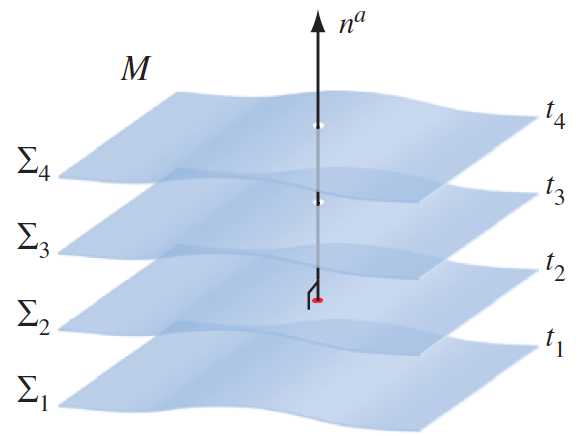
\includegraphics[width=8cm,height=5cm]{figs/foliation.png}
  \caption{The spacetime $M$ is foliated by the spacelike hypersurfaces $\Sigma_t$. At each point on a spacelike hypersurface, a unit normal vector $n^\alpha$ is defined. Figure from \cite{Baumgarte2010}.}
\end{figure}

\vskip0.5cm
{\bf Exercise 9.1:} Derive the following explicit components for $t^\alpha$, $n^\alpha$, $\beta^\alpha$ and $\gamma_{ij}$ 
\bea 
t^\mu &=& (1,0,0,0),\\
t_{\mu} &=& (-\alpha^2+\b_i \b^i, \b_i), \\
n^\mu &=& \frac{1}{\alpha} \cdot ( 1 ,  - \beta ^ { i }  ), \\
n_\mu &=& -\alpha \cdot(1,0,0,0), \label{nmu} \\
\beta^t & = & 0, \\
\beta_t & = & \b_i \b^i, \\
\beta_i &=& \gamma_{ij}\beta^j,\\
\gamma_{tt} & = & g_{tt}+\alpha^2, \\
\gamma_{ti} & = & g_{ti}, \\
\gamma_{ij}  &=&  g_{ij},
\eea
and show that 
\be
\sqrt{-\na_\b t\na^\b t} = \alpha^{-1}.
\ee

\vskip0.5cm
Notice that $\gamma_{ij}$ is simply the {\it spatial part} of $g_{\mu\nu}$. Furthermore, it follows that
\be
 g_{tt} = t_\a t^\a=-\a^2+\b_i \b^i.
 \ee
 and thus
 \be
 \gamma_{tt} =\b_i \b^i.
 \ee
 and by the definition (\ref{shift}), the covariant component of the shift vector is 
 \be
 \beta_i = \gamma_{ti}.
 \ee
 
Combining the above results, it follows immediately that the metric element is written as
\be
\boxed{ ds^2 = -\alpha^2 dt^2 +\gamma_{ij}(dx^i+\beta^i dt)(dx^j+\beta^j dt)
}.
\label{gmunu}
\ee
corresponding to the mentric tensor 
\be
g _ { \mu \nu } = \left( \begin{array} { c c } { - \alpha ^ { 2 } + \beta _ { k } \beta ^ { k } } & { \beta _ { i } } \\ { \beta _ { j } } & { \gamma _ { i j } } \end{array} \right).
\ee
The inverse metric tensor is
\be
g ^ { \mu \nu } = \left( \begin{array} { c c } { - 1 / \alpha ^ { 2 } } & { \beta ^ { i } / \alpha ^ { 2 } } \\ { \beta ^ { j } / \alpha ^ { 2 } } & { \gamma ^ { i j } - \beta ^ { i } \beta ^ { j } / \alpha ^ { 2 } } \end{array} \right).
\ee

\begin{figure}
  \centering
  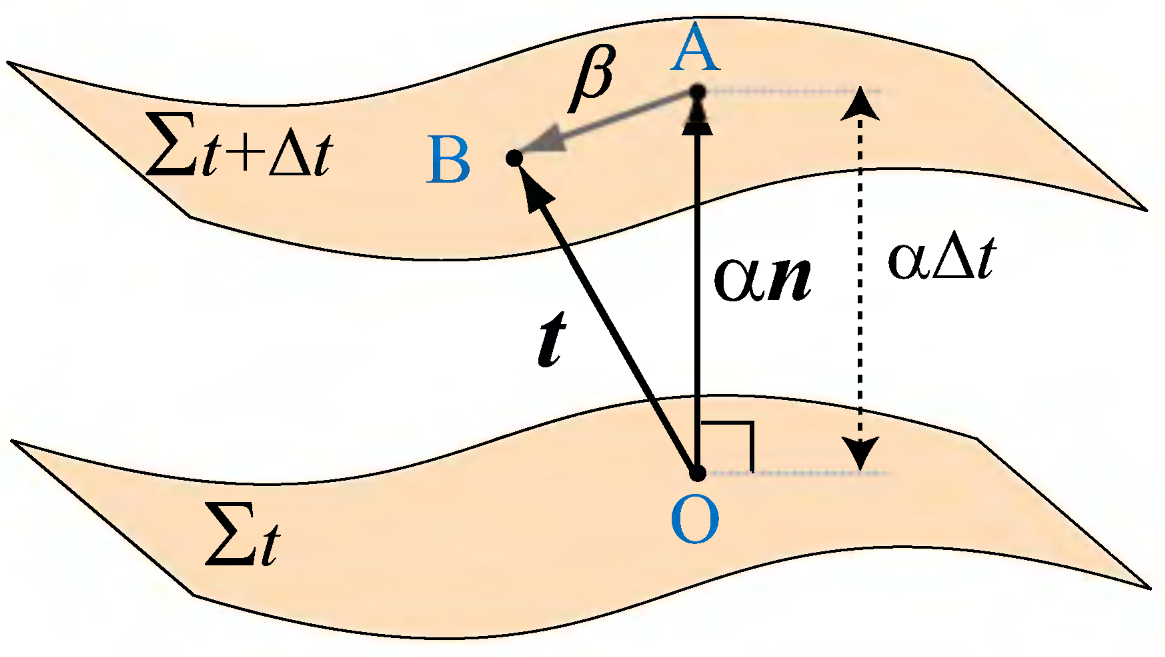
\includegraphics[width=8cm,height=5cm]{./figs/Lapse-Shift.png}
  \caption{The timelike vector field $t^\alpha$ (connecting points of fixed coordinates $x^i$ on different hypersurfaces) is, in general, decomposed into  $\alpha n^\alpha$ (normal to $\Sigma_t$) and $\beta^\alpha$ (tangent to  $\Sigma_t$). The proper time elapsed between the two hypersurfaces is $\alpha \Delta t$.  Figure from \cite{Shibata1996}.}
\end{figure}


\section{The induced metric}

The {\it pullback} of $\gamma_{\alpha \beta}$ to $\Sigma_t$ is the 3-dimensional tensor 
\be 
\boxed{ \gamma_{ab} = \gamma^\alpha{}_a \,\gamma^\beta{}_b \,\gamma_{\alpha\beta}},\ee
 which is the Riemannian 
{\it 3-metric}, or {\it induced metric} on $\Sigma_t$.  In the charts 
$\{x^i\}$ for $\Sigma_t$ and $\{t,x^i\}$ for spacetime $M$, $\gamma^\alpha{}_a$
has components
\be
   \gamma^\mu{}_i = \delta_i^\mu,
\ee
because $n_i=0$. The spatial components of 
$\gamma_{ab}$, $\gamma_{\a\b}$ and $g_{\a\b}$ 
all coincide:
\be 
 \gamma_{ij} = g_{ij}.
\ee 
Similarly, the pullback of  $\beta_\alpha$ on $\Sigma_t$ is 
\be
\boxed{ \beta_a = \gamma^\alpha{}_a \,\beta_\alpha },
\ee
which is a 3-dimensional covariant vector on $\Sigma_t$. Defining the determinant of the 3-metric as $\c={\rm det}(\g_{ab})$, the
volume element is
\be
\sqrt{|g|}= \alpha\sqrt\gamma.
\ee

The choice of a 3+1 decomposition ${\mathbb R}\times \Sigma$ 
of the spacetime allows one to identify each hypersurface $\Sigma_t=\{t\}\times \Sigma$ with 
the fixed space $\Sigma$.  We can then regard $\alpha(t)$, $\beta^a(t)$, 
$\gamma_{ab}(t)$, and the 3-dimensional projections of the fluid variables 
as time-dependent quantities on $\Sigma$.   

The correspondence between fields $\alpha(t), \beta^a(t)$, 
and $\gamma_{ab}(t)$ on $\Sigma$ and $\alpha,\beta^\a$, and $\gamma_{\a\b}$ on $M$ extends 
to a correspondence between the time derivatives $\dot\a =\pa_t\a$, $\dot\beta^a=\pa_t\beta^a$, $\dot\g_{ab}=\pa_t\g_{ab}$ on $\Sigma$ and the Lie derivatives $\dot\a = \Lie_{\bm t}\a$, $\dot\beta^\a=\Lie_{\bm t}\beta^\a$, $\dot\g_{\a\b}=\Lie_{\bm t}\g_{\a\b}$ on $M$. For example, 
\be
 \dot\gamma_{ab} := \partial_t\gamma_{ab} = \g^\a{}_a\g^\b{}_b \Lie_{\bm
t} 
 \gamma_{\a\b}=\g^\a{}_a\g^\b{}_b \dot \gamma_{\a\b}.
\ee 
This follows immediate from the fact that the spatial components of corresponding tensors 
coincide. 
  


  

The pullback of the covariant derivative operator $\nabla_\alpha$ on $\Sigma$ is 
\be
D_a = \gamma^\alpha{}_a\nabla_\alpha.
\ee
   and the \textit{extrinsic curvature}  $K_{ab}$ of $\Sigma$ is defined as\footnote{There is no consistent convention in the literature for 
the sign of the extrinsic curvature of a spacelike hypersurface.  
Our convention agrees with that of MTW \cite{MTW} and disagrees with 
Wald's \cite{waldbook}.}
\be
\boxed{ K_{ab} := -\frac12\gamma^\a{}_a \gamma^\b{}_b \Lie_{\bf n} \gamma_{\a\b}},
\label{eq:kab0}\ee 
which can be regarded (up to a factor of -1/2) as a "time-derivative" along the normal $n^\alpha$. The contraction $K$ of the extrinsic curvature is 
\be
K=K_a{}^a = \gamma^{ab}K_{ab}.
\ee
\vskip0.5cm

\noindent {\bf Exercise 10.1:} Using Eqs.~(\ref{eq:kab0}) and (\ref{eq:ta}), show that 
\bea
 K_{ab} &=& -\frac12\gamma^\a{}_a \gamma^\b{}_b \Lie_{\bf n} \gamma_{\a\b}
 = -\frac1{2\alpha} [\partial_t \gamma_{ab}
          -\gamma^\alpha{}_a \gamma^\beta{}_b (\nabla_\a \b_\b + \nabla_\b \b_\a)]
\nonumber\\
 &=& -\frac1{2\alpha} (\partial_t \gamma_{ab}
          -D_a \b_b - D_b \b_a).
\label{eq:gabevol0}\eea 

\vskip0.5cm 
Eq.~(\ref{eq:gabevol0}), in the form
\index{Einstein field equation!evolution equations|(}
\be
\boxed{\partial_t \gamma_{ab} = -2\a K_{ab} +D_a \b_b + D_b \b_a},
\label{eq:gabevol}\ee
serves as an evolution equation for the 3-metric $\gamma_{ab}$. 

The energy density  $\rho_{\rm E}$,
the momentum density $j_a$, and the stress tensor {\it $S_{ab}$ as measured by an observer
whose 
4-velocity is $n^\alpha$} are  
\bsube\bea
  \rho_E &:=& n^\a n^\b T_{\a\b} = (\epsilon+p)(\alpha u^t)^2-p,\\
  j_a    &:=& -\g_a{}^\a n^\b T_{\a\b} = (\epsilon+p) \alpha u^t u_a, \\
  S_{ab} &:=& \g_a{}^\a \g_b{}^\b T_{\a\b} 
        = (\epsilon+p) u_a u_b + p\gamma_{ab}, 
\eea\label{eq:tdecomp}
\esube 
\noindent where $u_a = \gamma^\a{}_a u_\a$. 
We denote by $R_{ab}$ the \textit{3-dimensional 
Ricci tensor of the 3-metric} $\gamma_{ab}$ and by 
\be
        R = \gamma^{ab}R_{ab},
\ee
the corresponding \textit{3-dimensional Ricci scalar}.  The 4-dimensional Ricci scalar 
will be written $^4\!R$.  

The field equation \mbox{$E^{\a\b}:=G^{\a\b}-8\pi T^{\a\b}=0$} can be decomposed in terms of components that are either entirely tangent to  $\Sigma_t$, or entirely normal to $\Sigma_t$ as well as in terms of mixed components. The
projection that is entirely tangent to  $\Sigma_t$, which is
$E_\parallel^{\a\b} \equiv \gamma^\a{}_\c \gamma^\b{}_\d E^{\c\d}=0$, 
has the form
\be
\boxed{\partial_t K_{ab} = -D_{a}D_{b}\alpha 
+ \alpha ( R_{ab} + K K_{ab}  - 2 K_{ac}K^{c}{}_{b})
+ \Lie_{\bm \b}K_{ab} 
 -8\pi\alpha\left[S_{ab}-\frac{\gamma_{ab}}{2}(S_c{}^c-\rho_{\rm E})
\right]},
\label{eq:Kabevol}
\ee
which is as evolution equation for $K_{ab}$.

The projection that is entirely normal to $\Sigma_t$, which is $E_{\perp\perp}\equiv E^{\a\b}n_\a n_\b=0$, is the {\it Hamiltonian constraint} 
\be
\boxed{ R+K^2-K_{ab}K^{ab}-16\pi\rho_{\rm E} = 0}, 
\index{Hamiltonian constraint}\label{eq:Hamconstraint}
\ee
whereas the mixed projection,
$E^a_{\parallel\perp}\equiv E^{\a\b}\g^a{}_\a n_\b=0$, is the {\it momentum constraint}
\be 
\boxed{D_b(K^{ab}-\gamma^{ab}K) -8 \pi j^a = 0}. 
\index{Momentum constraint}\label{eq:momconstraint}
\ee


The system of equations (\ref{eq:gabevol}), (\ref{eq:Kabevol}) describes the time 
evolution of the three-dimensional tensor fields $\g_{ab}(t)$ 
and $K_{ab}(t)$ on $\Sigma$.  Since these equations
do not contain time derivatives of
the lapse function $\alpha$ or of the shift vector $\beta^a$, these 
metric functions are not dynamical variables. One can regard the four degrees 
of gauge freedom associated with the choice of coordinates $(t, x^i)$ as 
the freedom to choose $\alpha$ and $\beta^a$.  Once $\alpha$ and $\beta^a$ are prescribed, one needs initial data  $\gamma_{ab}(0)$ and $K_{ab}(0)$  satisfying
the constraint equations (\ref{eq:Hamconstraint},\ref{eq:momconstraint}).

Next, we consider the 3+1 decomposition of the conservation equations governing the fluid. Baryon conservation (\ref{eq:baryon}), has the form 
$0 = \na_\a(\rho u^\a\sqrt{|g|}) = \partial_\mu(\rho u^\mu\sqrt{|g|})$.
The upper and lower components are related by 
$u_i = \gamma_{i\mu} u^\mu = \gamma_{ij}u^j + \beta_i u^t$, 
or 
\be
   u^i = \gamma^{ij}u_j -\beta^i u^t.    
\ee

The difference is related to the relation between decompositions with 
$n^\a$ and with $t^\a= \a n^\a + \b^\a$ as the timelike vector.  To write this relation, 
we introduce the 3-velocity $v_a$ measured by an observer with velocity $n^\alpha$.    
Using the correspondence $v_a=\gamma_a{}^\a v_\a$ between $v_a$ and a 4-vector 
$v_\a$ for which $v_\a n^\a=0$, we have    
\be
   u_\alpha = W (n_\alpha + v_\alpha),  
\label{eq:u3+1}\ee
where $u^\a u_\a = -1$ implies that $W$ is the Lorentz factor  
\be
   W = \frac1{\sqrt{1-v^2}}, 
\label{eq:ww}\ee
with $v^2 = v^\a v_\a = \gamma_{ab}v^a v^b$.  
Using Eqs.~(\ref{eq:contrametric}) and (\ref{eq:tmu}), we can write the components of Eq.~(\ref{eq:u3+1}) 
as 
\be
    W = \alpha u^t, \quad 
        u^i = u^t\left(\a v^i -\b^i\right), 
\label{eq:wv}\ee 
and the decomposition of $u^\a$ with respect to $t^\a$ is 
\be
u^\a = u^t(t^\a + \a v^\a -\beta^\a).
\ee


The evolution of a perfect fluid is governed by conservation of baryons (the continuity equation), (\ref{eq:baryon}), the Euler equation, (\ref{eq:euler}), and conservation of energy, (\ref{econs}), together with an equation of state.  These first three equations have the 3+1 form 
\bea
  \pa_t(\rho\, u^t\alpha \sqrt{\gamma}) 
                &=& -  D_b [\rho u^t(\a v^b-\b^b)\,\sqrt{\gamma}],
\label{eq:bcons3+1}\\
  \pa_t j^a &=& \Lie_{\bm\beta} j^a +\a(2K^a{}_b+\delta^a_b K) j^b 
                - D_b(\alpha S^{ab}) -\rho_E D^a \alpha.\qquad
\label{eq:euler3+1}\\
 \pa_t \rho_E &=& \Lie_{\bm\beta} \rho_E +\alpha K\rho_E -\frac1\alpha D_b(\alpha^2 j^b) +\alpha K_{ab}S^{ab}.
\label{eq:econs3+1}
\index{perfect fluid!evolution equations}\index{Euler equation!relativistic}\eea  
\index{evolution equations!fluid}\index{continuity equation}

For a one-parameter equation of state, $\epsilon = \epsilon(\rho), \, 
p = p(\rho)$,  satisfying the zero-entropy first law of thermodynamics, (\ref{eq:dedrho}), 
the energy conservation equation, (\ref{eq:econs3+1}), is redundant, implied by baryon conservation and the equation of state. The evolution of the fluid is then 
given by Eqs.~(\ref{eq:bcons3+1}), (\ref{eq:euler3+1}), and the equation 
of state.
%
Initial data for the fluid are the values 
of baryon mass density $\rho$ and fluid 3-velocity $u^a$, with initial values of 
$\epsilon$, $p$ and $u^t$ determined by the equation of state 
and the normalization $u_\alpha u^\alpha= -1$.   

% The time-evolution is then determined by the evolution equations 
% (\ref{eq:gabevol}) and (\ref{eq:Kabevol}), whose components constitute a 
% system of six first-order (in time) evolution equations for six components
% of $\gamma_{ab}$. 
A solution $\g_{ab}(t), K_{ab}(t),\alpha(t), \beta^a(t), \epsilon(t), p(t), u^a(t)$ to 
the Einstein-Euler system, in the decomposed form 
(\ref{eq:gabevol}), (\ref{eq:Kabevol})-(\ref{eq:euler3+1}), then yields 
the four-dimensional metric (\ref{gmunu}) whose source is a perfect fluid 
having 4-velocity $u^\a = u^t( t^\a+\gamma^\a{}_a u^a)$.  
In solving the system numerically, one specifies initial 
data satisfying the constraint equations at $t=0$; and one essentially solves 
only the evolution equations, (\ref{eq:gabevol}), (\ref{eq:Kabevol}), for the metric 
and (\ref{eq:bcons3+1}), (\ref{eq:euler3+1}) for the fluid.  The resulting 
evolution then preserves the constraints: Eqs.~(\ref{eq:Hamconstraint}) and 
(\ref{eq:momconstraint}) are automatically satisfied.  Preservation of the 
constraints is a consequence of the Bianchi identity, $\nabla_\b G^{\a\b}=0$, 
and the fluid equation $\nabla_\beta T^{\a\b}=0$, because the equation 
$\nabla_\b(G^{\a\b}-8\pi T^{\a\b})=0$ expresses the time derivative of 
the constraint $(G^{\a\b}-8\pi T^{\a\b})n_\a$ at a time $t$ 
in terms of the field equation and its spatial derivatives at $t$.  

The time evolution of a fluid with smooth initial data is, in general, 
smooth for a finite time (see below), after which shock waves appear\index{shocks}.
Within a perfect-fluid description, shocks are solutions in which the 
fluid variables are discontinuous on a characteristic hypersurface -- 
the history of a two-surface that moves at the speed of sound.     
Formally maintaining a one-parameter equation of state can be appropriate for 
solutions without shocks or with small shocks; but it is not appropriate 
for strong shocks, because it ignores the heat generated by the shock.  
There is, however, a common approximation that roughly accounts for the heat 
generated without introducing the complications of neutrino and radiative 
transport.  One adopts a two-parameter EOS of the form (\ref{eqsti}), and 
uses the continuity and energy conservation equations, (\ref{eq:bcons3+1}) and 
(\ref{eq:econs3+1}), as independent evolution equations for $\rho$ and $\epsilon$.  
With no shocks, as we have just seen, this evolution preserves the thermodynamic 
relation (1st law) between $\epsilon$ and $\rho$ that maintains a constant-entropy 
equation of state, 
$\epsilon = \epsilon(\rho)$.  \index{equation of state!two-parameter}
When there are shocks,
the constant-entropy first law is violated by the time evolution. The evolution 
equations again determine $\epsilon$ and $\rho$, but $\epsilon$ is
 no longer a one-parameter function $\epsilon(\rho)$.  
% The pressure is always given by
% $p = p_cold(rho)+ p_th[epsilon-epsilon_P(rho)]$, where
% $p_th(epsilon) = (Gamma_th -1) epsilon$, with $Gamma_th = 1.5$.
% [Note that epsilon here has the meaning of $\rho\varepsilon$
% in Phys. Rev. D 67, 024033 (2003).]
 
\index{Einstein field equation!existence of solutions}       
For both numerical evolution and for proving existence of solutions, 
it is important to note that the system as described is not strongly 
hyperbolic.  To turn it into a strongly hyperbolic system one can 
add to the dynamical equations linear combinations of the constraint 
equations 
%(the BSSN method \cite{bssn,lindblomxx}) 
 or use harmonic 
coordinates, coordinates for which $\partial_\nu ( g^{\mu\nu}\sqrt{|g|}) = 0$
(see also Sect.~\ref{sec:ghc} for generalized version). 
The harmonic gauge condition, in effect, replaces spatial derivatives in the 
constraint equations by time derivatives and leaves each component of
the Ricci tensor in the manifestly hyperbolic form
$R_{\mu\nu}= -\frac12 g^{\sigma\tau}\pa_\sigma\partial_\tau g_{\mu\nu} 
+ F_{\mu\nu}(\partial g, g)$. With this form, local existence of solutions 
to the vacuum Einstein equation for analytic data is immediate from the 
Cauchy-Kovalevskaya theorem (see \cite{Courant1962}) and was first 
proved for smooth data by Choquet-Bruhat \cite{Choquet-Bruhat1956}:
For any smooth initial data $(\gamma_{ab}, \partial_t\gamma_{ab})$
on a hypersurface $\Sigma$ there is a solution $g_{\a\b}$ to the 
vacuum Einstein equation in a neighborhood of $\{0\}\times\Sigma$ in
$M={\mathbb R}\times\Sigma$, and the solution is unique up to isometry.
Local existence for perfect fluids without boundary was proved by 
Lichnerowicz \cite{lichnerowicz67}, but for local evolution of stars, 
modeled as perfect fluids with boundary in an asymptotically flat 
spacetime, there is still no proof available (see 
\cite{Choquet-Bruhat1980,Rendall2005} for reviews of the Cauchy problem). 
Proof of existence of solutions with shocks (weak solutions to the Einstein-Euler system
in which the fluid variables are discontinuous)  is so far restricted to a few 
equations of state and to a few symmetric spacetimes \cite{gst07,ls05,blss04}.
\index{initial value problem|)}\index{shocks}

\section{The CFC approximation}

Following Wilson et al. (1996) (see also Flanagan 1999; Mathews \& Wilson 2000) we approximate the general metric $g_{\mu\nu}$ by replacing its spatial three-metric $\gamma_{ij}$ with the conformally flat (CF) three-metric (conformal flatness condition ? CFC hereafter):

\begin{equation}
\gamma_{i j}=\phi^{4} \hat{\gamma}_{i j}
\end{equation}

where $\hat \gamma_{ij}$ is the flat metric ($\hat \gamma^{ij}=\delta_{ij}$ in Cartesian coordinates). In general, the conformal factor $\phi$ depends on the coordinates $x^i$. Therefore, at all times during a numerical simulation we assume that all off-diagonal components of the three-metric are zero, and the diagonal elements have the common factor $\phi^4$. Note that all metric quantities with a hat are defined with respect to the flat three-metric $\hat \gamma_{ij}$.

Within this approximation the ADM equations reduce to a set of five coupled elliptic (Poisson-like) equations for the metric components,

\begin{eqnarray}
\hat{\Delta} \phi &=&-2 \pi \phi^{5}\left(\rho h W^{2}-P+\frac{K_{i j} K^{i j}}{16 \pi}\right), \\
\hat{\Delta}(\alpha \phi) &=&2 \pi \alpha \phi^{5}\left(\rho h\left(3 W^{2}-2\right)+5 P+\frac{7 K_{i j} K^{i j}}{16 \pi}\right),\\
\hat{\Delta} \beta^{i} &=&16 \pi \alpha \phi^{4} S^{i}+2 \hat{K}^{i j} \hat{\nabla}_{j}\left(\frac{\alpha}{\phi^{6}}\right)-\frac{1}{3} \hat{\nabla}^{i} \hat{\nabla}_{k} \beta^{k},
\end{eqnarray}

where $\hat\nabla$ and   $\hat\Delta$ are the flat space Nabla and Laplace operator, respectively. The transformation behavior between the extrinsic curvature defined on $\gamma_{ij}$ and $\hat \gamma_{ij}$  is as follows:

\begin{equation}
K_{i j}=\phi^{-2} \hat{K}_{i j}, \quad K^{i j}=\phi^{-10} \hat{K}^{i j}.
\end{equation}

The metric Eqs. (7)?(9) couple to each other via their right hand sides, and in case of the equations for $\beta^i$ via the operator $\hat\Delta$ acting on the vector $\beta^i$ . The equations are dominated by the source terms involving the hydrodynamic quantities $\rho, P$ and $v^i$, whereas the nonlinear coupling through the other, purely metric, source terms becomes only important for strong gravity. On each time slice the metric is solely determined by the instantaneous hydrody- namic state, i.e. the distribution of matter in space.


\newpage

\section{Linear Perturbations and Gravitational Waves}

Assume a metric  $g_{\mu\nu}$, that differs from Minkowski metric $\eta_{\mu\nu}$ as
\begin{equation}
\boxed{g_{\mu\nu}=\eta_{\mu\nu}+h_{\mu\nu}},
\end{equation}
with $ |h_{\mu\nu} |\ll 1 $. Using the flat metric tensor, one can define  \begin{equation}
 h_{\mu}{}^{\nu} \equiv \eta^{\nu\beta} h_{\mu\beta},
 \end{equation}
\begin{equation}
 h^{\mu\nu} \equiv \eta^{\mu\alpha} \eta^{\nu\beta} h_{\alpha\beta},
 \end{equation}
 \begin{equation}
 h \equiv h^\alpha{}_{\alpha}=\eta^{\mu\alpha}  h_{\mu\alpha}.
 \end{equation}
The metric must satisfy
\begin{equation}
 g_{\mu\nu} g^{\nu\beta} =(\eta_{\mu\nu}+h_{\mu\nu})(\eta^{\nu\beta}+\delta g^{\nu\beta})=\delta_{\mu}^{\beta},
 \end{equation} 
 which leads to 
\begin{equation}
 \delta g^{\mu\nu}=-h^{\mu\nu}.
 \end{equation}
 In order to derived the linearized Riemann tensor, we first need to linearize the Christoffel symbols. In a chosen coordinate system, the Christoffel symbols can be expressed as
\begin{equation}
\Gamma_{\alpha \beta}^{\mu}=\frac{1}{2} g^{\mu \nu}\left(g_{\nu \alpha, \beta}+g_{\beta \nu, \alpha}-g_{\alpha \beta, \nu}\right).
\end{equation}
The perturbation of the partial derivatives of the metric are, e.g.
$$
(\delta g_{\nu \alpha})_{, \beta}=\eta_{\nu \alpha, \beta}+h_{\nu \alpha, \beta}=h_{\nu \alpha, \beta}.
$$
The linearized Christoffel symbols are then
$$
\begin{aligned} \delta \Gamma_{\alpha \beta}^{\mu} &=\frac{1}{2} \eta^{\mu \nu}\left(h_{\nu \alpha, \beta}+h_{\beta \nu, \alpha}-h_{\alpha \beta, \nu}\right), \\ &=\frac{1}{2}\left(h_{\alpha}{}^{\mu}{}_{, \beta}
+ h_{\beta}{}^{\mu}{}_{, \alpha} - h_{\alpha\beta}{}^{,\mu}{}\right).
 \end{aligned}
$$
The linearized Riemann tensor is
simply\begin{eqnarray}
\delta R_{\alpha\mu\beta\nu} & \equiv & \frac{1}{2} \delta (g_{\alpha\nu,\mu\beta}-g_{\alpha\beta,\mu\nu}+g_{\mu\beta,\alpha\nu}-g_{\mu\nu,\alpha\beta}),\nonumber
\\
& = & \frac{1}{2}(h_{\alpha\nu,\mu\beta}-h_{\alpha\beta,\mu\nu}+h_{\mu\beta,\alpha\nu}-h_{\mu\nu,\alpha\beta}),
\end{eqnarray}
the linearized Ricci tensor is


\begin{eqnarray}
\delta R_{\mu\nu}=\eta^{\alpha\beta} \delta R_{\alpha\mu\beta\nu} & = & \frac{1}{2}\eta^{\alpha\beta}(h_{\alpha\nu,\mu\beta}-h_{\alpha\beta,\mu\nu}+h_{\mu\beta,\alpha\nu}-h_{\mu\nu,\alpha\beta}),\nonumber\\
& = & \frac{1}{2}(h_{\nu}{}^{\alpha}{}_{,\mu\alpha}-h_{,\mu\nu}+h_{\mu}{}^{\alpha}{}_{,\alpha\nu}-h_{\mu\nu,\alpha}^{\phantom{\mu\nu,\alpha}\alpha}),
\end{eqnarray} 
and the linearized Ricci scalar is 
\begin{eqnarray}
\delta R = \eta^{\mu\nu}\delta R_{\mu\nu}.
\end{eqnarray}
Then, the linearized field equations become
$$
h_{\mu \alpha,}{}^{\alpha}{}_{ \nu}+h_{\mu \alpha,}{}^{\alpha}{}_{\mu}-h_{\mu \nu,}{}^{\alpha}{}_ \alpha - h_{, \mu \nu}-\eta_{\mu \nu}
\left(h_{\alpha \beta,}{}^{\alpha \beta}-h_{,}{}_{ \alpha}{}^{\alpha}\right)=16 \pi \delta T_{\mu \nu}
$$ 
 
The wave-like character of the linearized field equations is more clearly revealed if one works with the \textit{trace-reversed} perturbation 
$$
\bar{h}_{\mu \nu} \equiv h_{\mu \nu}-\frac{1}{2} \eta_{\mu \nu} h,
$$
for which $\bar h=-h$. Then, the linearized field equations become
$$
-\bar{h}_{\mu \nu, \alpha}{}^{\alpha}-\eta_{\mu \nu} \bar{h}_{\alpha \beta,}{}^{\alpha \beta}+\bar{h}_{\nu \alpha,}{}^{\alpha}{}_{ \mu}=16 \pi \delta T_{\mu \nu}.
$$
The first term can be written using the short-hand notation for the d'Alembertian (wave) operator
\begin{eqnarray}
\square & = & \eta^{\alpha\beta} \partial_{\alpha}\partial_{\beta}\nonumber\\
& = & \partial_{\alpha}\partial^{\alpha}\nonumber\\
& = & -\frac{\partial^{2}}{\partial t^{2}}+\nabla^{2}\nonumber,
\end{eqnarray}
so that 
$$
\boxed{-\square \bar{h}_{\mu \nu}-\eta_{\mu \nu} \bar{h}_{\alpha \beta,}{}^{\alpha
\beta}+\bar{h}_{\nu \alpha,}{}^{\alpha}{}_{ \mu}=16 \pi \delta T_{\mu \nu}}.
$$
which is more compact than the original equation. As we will see next, the second and third terms on the left side can be eliminated by an infinitesimal coordinate transformation. 
\subsection{Gauge freedom for infinitesimal perturbations}Linear perturbations of a spacetime metric have a gauge freedom to infinitesimal transformations of the coordinates,
of the form
\begin{equation}
x^{\alpha '}=x^{\alpha}+\xi^{\alpha},
\end{equation}
where $\xi^\alpha$ is an infinitesimal displacement. In the new coordinate system, the metric becomes
\begin{equation}
g'_{\mu\nu}(x')=\frac{\partial x^{\alpha}}{\partial x'^{\mu}} \frac{\partial
x^{\beta}}{\partial x'^{\nu}} g_{\alpha\beta}(x).
\end{equation}
Since
\begin{equation}
\frac{\partial x^{\alpha}}{\partial x'^{\beta}}=\delta_{\beta}^{\alpha}-\xi^{\alpha}_{\phantom{\alpha},\beta},
\end{equation}
it follows that
\begin{eqnarray}
g'_{\mu\nu} & = & (\delta_{\mu}^{\alpha}-\xi^{\alpha}_{\phantom{\alpha},\mu})(\delta_{\nu}^{\beta}-\xi^{\beta}_{\phantom{\beta},\nu})(\eta_{\alpha\beta}+h_{\alpha\beta}),\nonumber\\
& = & \eta_{\mu\nu}+h_{\mu\nu}-\delta_{\nu}^{\alpha}\eta_{\alpha\beta}\xi^{\beta}_{\phantom{\beta},\nu}-\delta_{\nu}^{\beta}\eta_{\alpha\beta}\xi^{\alpha}_{\phantom{\alpha},\mu}+\mathscr{O}[\xi^{2},\xi
\cdot h],\nonumber\\
& = & \eta_{\mu\nu}+h_{\mu\nu}-\xi_{\mu,\nu}-\xi_{\nu,\mu},
\end{eqnarray}
and the two metric perturbations are related as
\begin{equation}
h'_{\mu\nu}=h_{\mu\nu}-\xi_{\mu,\nu}-\xi_{\nu,\mu}.
\label{eq:guagetrans}
\end{equation}
The infinitesimal displacement vector can then be suitably chosen to enforce a certain gauge condition. Choosing the four components of $\xi^\alpha$ is equivalent to specifying four conditions on the components of $\bar{h}_{\mu\nu}$. 

In terms of the traceless metric perturbation $\bar{h}^{\mu \nu}$, Eq. (\ref{eq:guagetrans}) becomes
\begin{equation}
\bar{h^{\prime}}^{\mu \nu}=\bar{h}^{\mu \nu}-\xi^{\mu, \nu}-\xi^{\nu, \mu}+\eta^{\mu
\nu} \xi^{\alpha}{}_{, \alpha},
\end{equation}
and taking a derivative, one obtains
\begin{equation}
\bar{h^{\prime}}^{\mu \nu}{}_{,\nu}=\bar{h}^{\mu \nu}{}_{,\nu}- \square\xi^{\mu}.
\end{equation}

\subsection{Lorentz Gauge}
The linearized field equations simplify considerably, if one transforms to a new coordinate system $x'$, in which \begin{equation}
{\overline h'}^{\mu\nu}_{\phantom{\mu\nu},\nu}=0,
\label{eq:Lorentzgauge}
\end{equation}
\begin{equation}
\Rightarrow \ \ \ \square \xi^{\mu}={\overline
h}^{\mu\nu}_{\phantom{\mu\nu},\nu} \equiv f^{\mu}(x).
\end{equation}
The latter is an inhomogeneous wave equation, with source $f^\mu(x)$. The d'Alembertian operator is invertible, having a Green's function $G(x-x')$, i.e.
\begin{equation}
\square_{x} G(x-x')=\delta^{4}(x-x'),
\end{equation}
with corresponding solution 
\begin{equation}
\xi^{\mu}(x)=\int d^{4} x 'G(x-x') f^{\mu}(x').
\end{equation}
One can thus always find an infinitesimal displacement to enforce the condition Eq. (\ref{eq:Lorentzgauge}). By analogy with electromagnetism, this condition is called the  Lorentz gauge (the correct name would be Lorenz gauge). It is the weak-field limit of the harmonic (or De-Donder) gauge in strong fields. 

But, notice that there exist trivial displacements, satisfying $\square \xi^{\mu}=0,$ that preserve the Lorentz gauge, since then
\begin{equation}
\bar{h^{\prime}}^{\mu \nu}{}_{,\nu}=\bar{h}^{\mu \nu}{}_{,\nu}=0.
\end{equation}
 A trivial displacement is thus a solution of $\square \xi^{\mu}=0,$ of the form
\begin{equation}
\xi^{\alpha}=C^{\alpha}e^{ik_{\mu}x^{\mu}},
\label{eq:trivial}
\end{equation}
where $k^\mu$ is a wave 4-vector and $C^\alpha$ is the amplitude 4-vector.

In vacuum, one can choose four arbitrary component of $\xi^\alpha$ and construct the tensor
\begin{equation}
\xi_{\mu \nu} \equiv  \xi_{\nu, \mu}+ \xi_{\mu, \nu}-\eta_{\mu \nu} \xi^{\rho}{}_{,\rho},
\end{equation}
which also satisfies $ \square \xi_{\mu \nu}=0 $, when $ \square \xi_{\mu }=0 $. By subtracting  $\xi_{\mu \nu}$  from $\bar h_{\mu\nu}$, one can impose four arbitrary conditions on the latter.

The initial 10 components of the perturbed metric $h_{\mu\nu}$ are reduced to just $10-4-4=2$ independent components, because of the general Lorentz gauge Eq. (\ref{eq:Lorentzgauge}) and of the freedom to specify the components of the 4-vector $C^\alpha$\ in Eq. (\ref{eq:trivial}}).


In the Lorentz gauge the linearized field equations become a simple wave equation
\begin{equation}
\square {\overline h}_{\mu\nu}=16\pi T_{\mu\nu}.
\end{equation}
In vacuum, one can show that $\square \bar h_{\mu\nu} = \square h_{\mu\nu} = 0$. Therefore, in vacuum the metric perturbations propagate as waves.

\subsection{The Transverse-Traceless Gauge}

In vacuum, one can choose $\xi^t$ so that
\begin{equation}
\boxed{\bar h =h=0},
\end{equation}
\begin{equation}
\Rightarrow \  \bar h_{\mu\nu} =h_{\mu\nu},
\end{equation}
which makes the perturbed metric \emph{traceless}. Next, one can choose the three spatial components $\xi^i$ in order to set
\begin{equation}
 \boxed{ \bar h^{ti} =0}.
\end{equation}
With the above choices, the $t$-component of the Lorentz gauge Eq. (\ref{eq:Lorentzgauge}) becomes
\begin{equation}
h^{tt}{}_{,t}=0,
\end{equation}
which means that $h_{tt}$ is constant in time (this corresponds to the static part of the gravitational interaction).
The gravitational wave itself corresponds to a time-dependent perturbation, so that for gravitational waves: 
\begin{equation}
\boxed{h^{tt}=0},
\end{equation}
which also implies that since the perturbed metric is traceless: 
\begin{equation}
\boxed{ h_i{}^i=0}.
\end{equation}
Finally, with the above choices, the spatial components of the Lorentz gauge  Eq. (\ref{eq:Lorentzgauge}) become\begin{equation}
\boxed{h^{i j}{}_{,j}=0}.
\end{equation}
The perturbed metric in this transverse-traceless gauge is denoted as $h_{ij}^{\rm TT}$ and contains only two remaining degrees of freedom. 

Notice that within the source, one can still choose a trivial displacement satisfying $\square \xi^{\mu}=0$ and construct a tensor satisfying
 $\square \xi_{\mu \nu}=0$, but now the wave equation has a source term, $\square {\overline h}_{\mu\nu}=16\pi T_{\mu\nu}$, so that by subtracting $\xi_{\mu\nu}$ from $\bar h_{\mu\nu}$, one cannot set to zero any further components.

\subsection{Plane waves}

The wave equation $\square \bar h_{\mu\nu} =0$ has plane wave solutions of the form 
\begin{equation}
\boxed{h_{i j}^{\mathrm{TT}}(x^\mu)=e_{i j}({k^i}) e^{i k_\alpha x^\alpha}},
\end{equation}
where is a null wave 4-vector ($k_\mu k^\mu=0$) with components $k^\mu=(\omega/c,k^i)$ and $\omega/c = \sqrt{k_i k^i}$.
The tensor $e_{i j}({k^i})$ is the \textit{polarization tensor}. For propagation along the $z-$axis, the polarization tensor in the TT gauge can be written as 
\begin{equation}
h_{i j}^{\operatorname{TT}}(t, z)=\left(\begin{array}{ccc}{h_{+}} & {h_{\times}} & {0} \\ {h_{\times}} & {-h_{+}} & {0} \\ {0} & {0} & {0}\end{array}\right)_{i j} \cos [\omega(t-z / c)],
\end{equation}
where $h_+$ and  $h_\times$ are the amplitudes of the "plus" and "cross" polarizations of the plane wave, respectively. Notice that the perturbation is nonzero only in the \textit{transverse} direction, with respect to the direction of propagation.

\section*{\\ Appendix}

\subsection*{Derivatives and integrals}
\index{integration}

The covariant derivative operator of the spacetime metric
$g_{\alpha\beta}$ will be written $\nabla_\alpha$, and the partial
derivative of a scalar $f$
with respect to one of the coordinates -- say r -- will be written
$\partial_r f$ or $f,_r$.  Lie derivatives along a vector $u^\alpha$
will be denoted by ${\cal L}_{\bf u}$.  The Lie derivative of an
arbitrary
tensor $T^{a\cdots b}{}_{c\cdots d}$ is
\ba
{\cal L}_{\bf u} T^{a\cdots b}{}_{c\cdots d} &=&
u^e\nabla_e T^{a\cdots b}{}_{c\cdots d}
-T^{e\cdots b}{}_{c\cdots d}\nabla_e u^a
- \cdots
- T^{a\cdots e}{}_{c\cdots d}\nabla_e u^b
 \nonumber \\
&&\phantom{u^e\nabla_e T^{a\cdots b}{}_{c\cdots d}}
+ T^{a\cdots b}{}_{e\cdots d}\nabla_c u^e+ \cdots
+ T^{a\cdots b}{}_{c\cdots e}\nabla_d u^e. \label{Lieiii}
\ea
Our notation for integrals is as follows.  We denote by $d^4V$ the
spacetime volume element.  In a chart $\{x^0, x^1, x^2, x^3\}$, the
notation 
means,
\be
d^4V = \epsilon_{0123} dx^0 dx^1 dx^2 dx^3 = \sqrt{|g|}\, d^4x,
\label{dtauii}
\ee
where $g$ is the determinant of the matrix $\|g_{\mu\nu}\|$. 
Gauss's theorem (presented in Sect. \ref{sec:gauss-stokes} of the Appendix) has the form
\be
\int_{\Omega} \nabla_\alpha A^\alpha d^4V= \int_{\partial\Omega} A^\alpha 
dS_\alpha,
\label{twth}
\ee 
with $\partial\Omega$ the boundary of the region $\Omega$. 
In a chart $(u, x^1, x^2, x^3)$ for which $V$ is a surface of
constant $u$, $ dS_\alpha = \sqrt{|g|}\; \nabla_\alpha u d^3x,$ and
\be
\int_V A^\alpha dS_\alpha = \int_V A^u \sqrt{|g|} d^3x  .\label{dSaii}
\ee
If $V$ is nowhere null, one can define a unit normal,
\be
\widehat n_\alpha = {{\nabla_\alpha u}\over{\big|\nabla_\beta u \nabla^\beta
u\big|^{1/2}}}\;,\label{na}
\ee
and write
\be  dS_\alpha = \widehat n_\alpha dV,
\ee
where
\be dV = \sqrt{|^3g|}\;d^3x,\label{dSaiii}
\ee
where ${}^3g$ is the determinant of the 3-metric induced on the surface $V$.
But Gauss's theorem has the form (\ref{twth})
for any 3-surface $S$, bounding a 4-dimensional region
${\cal R}$, regardless of whether $S$ is timelike, spacelike or null.%
\footnote{
Note that in the text, $n_\a$ denotes the {\em future} pointing unit normal
to a $t=$ constant hypersurface, $n_\a = -\na_\a t/|\na_\b t\na^\b t|^{1/2}$. 
In order that, for example, $\int \rho u^\a dS_\a$, be positive on a 
$t=$ constant surface, one must use $dS_\a = \na_\a t \sqrt{|g|}d^3x 
= \widehat n_\a dV = -n_\a dV$.}

Similarly, if $F^{\a\b}$ is an antisymmetric tensor, its integral over 
a 2-surface $S$ of constant coordinates $u$ and $v$ is written
\be
\int_S F^{\a\b} dS_{\a\b} = \int_S F^{uv} \sqrt{|g|}d^2 x,
\label{dSab}
\ee
and a corresponding generalized Gauss's theorem has the form
\be
\int_V \na_\b F^{\a\b} dS_\a = \int_{\partial V} F^{\a\b} dS_{\a\b}.
\label{eq:gauss0}
\ee
If $n_\a$ and $\widetilde n_\a$ are orthogonal unit normals to the 
surface $S$, for which $({\bf n, \widetilde n}, \bm\partial_2, \bm\partial_3)$ 
is positively oriented, then $dS_{\a\b} = n_{[\a}\widetilde n_{\b]} \sqrt{|^2g|}\, d^2x$.

\subsection*{Asymptotic notation: $O$ and $o$}
\index{$O(x)$, $o(x)$}
We will use the symbols $O(x)$ and $o(x)$ to describe asymptotic behavior 
of functions. For a function $f(x)$, $f=O(x)$ if there is a 
constant $C$ for which $ |f/x|<C$, for sufficiently small $|x|$; 
and $f=o(x)$ if $\lim_{x\rightarrow 0}|f/x|=0$. 
For example, if $A$ is constant, $A/r = O(r^{-1})$, 
and $A/r^{3/2} = o(r^{-1})$.  



\bibliography{bibliography}

\end{document}









